% IMPORTANT: PLEASE USE XeLaTeX FOR TYPESETTING
\documentclass[t]{sintefbeamer}
\usepackage{xeCJK}

% meta-data
\title{数据库系统概论}
\subtitle{第8章 数据库编程}
\author{黄俊杰}
\date{2023 Fall}
\titlebackground{images/background}

% \usepackage{zh_CN-Adobefonts_external}
\usetikzlibrary {%
arrows.meta,
backgrounds,
positioning,
fit,
petri,
shapes,
arrows,
snakes,
decorations,
external,calc,patterns,positioning,decorations.pathmorphing
}

\usepackage{booktabs}
\usepackage{multirow}

% \addtobeamertemplate{block begin}{%
%     \setlength{\textwidth}{0.8\textwidth}
% }{}



% document body
\begin{document}

\lstset{
    language=SQL,
    morekeywords={WITH,to_char,to_date,WHILE, LOOP, FOR, IF, ELSIF, DECLARE, CURSOR, OPEN, FETCH, EXIT, CALL, CLOSE, RAISE, NOTICE, PERFORM},
    numbers=left,
    stepnumber=1,
    linewidth=0.8\linewidth,
    xleftmargin=0.1\linewidth
}

\maketitle


\section{概述}
\subsection{1.1 SQL语言表达能力的限制}

\begin{frame}[fragile,allowframebreaks]{【任务1】打印课程的所有先修课}
\begin{itemize}
    \item 【任务1】打印“数据库系统概论”课程的所有先修课信息
    \begin{figure}
        \centering
        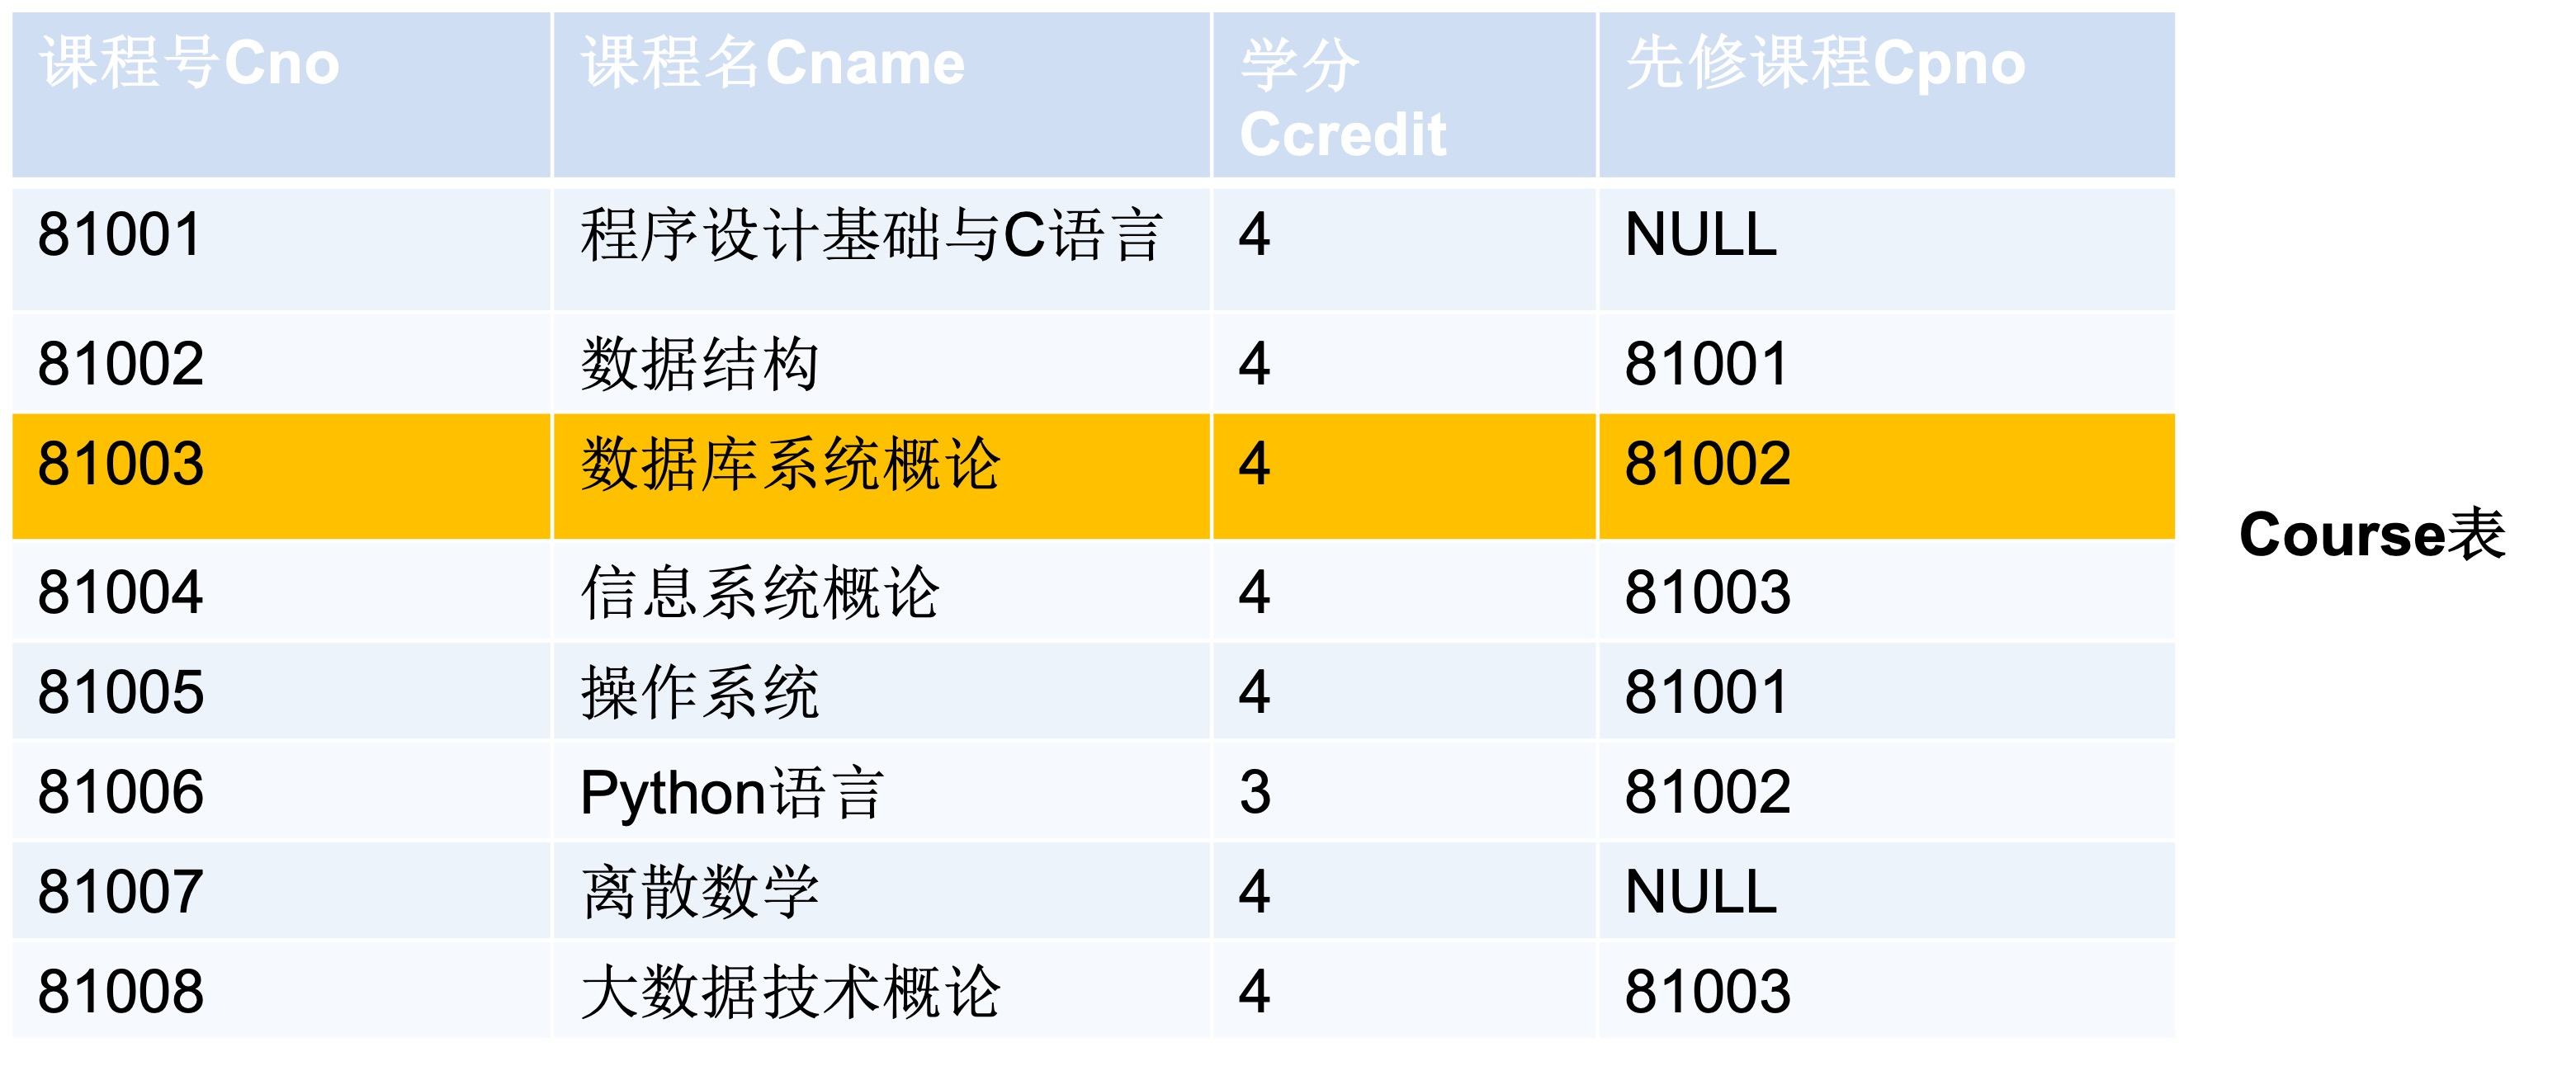
\includegraphics[width=0.8\textwidth]{figure/fig-1.jpg}
    \end{figure}
\framebreak
    
    \item【任务1】打印“数据库系统概论”课程的所有先修课信息

    \begin{figure}
        \centering
        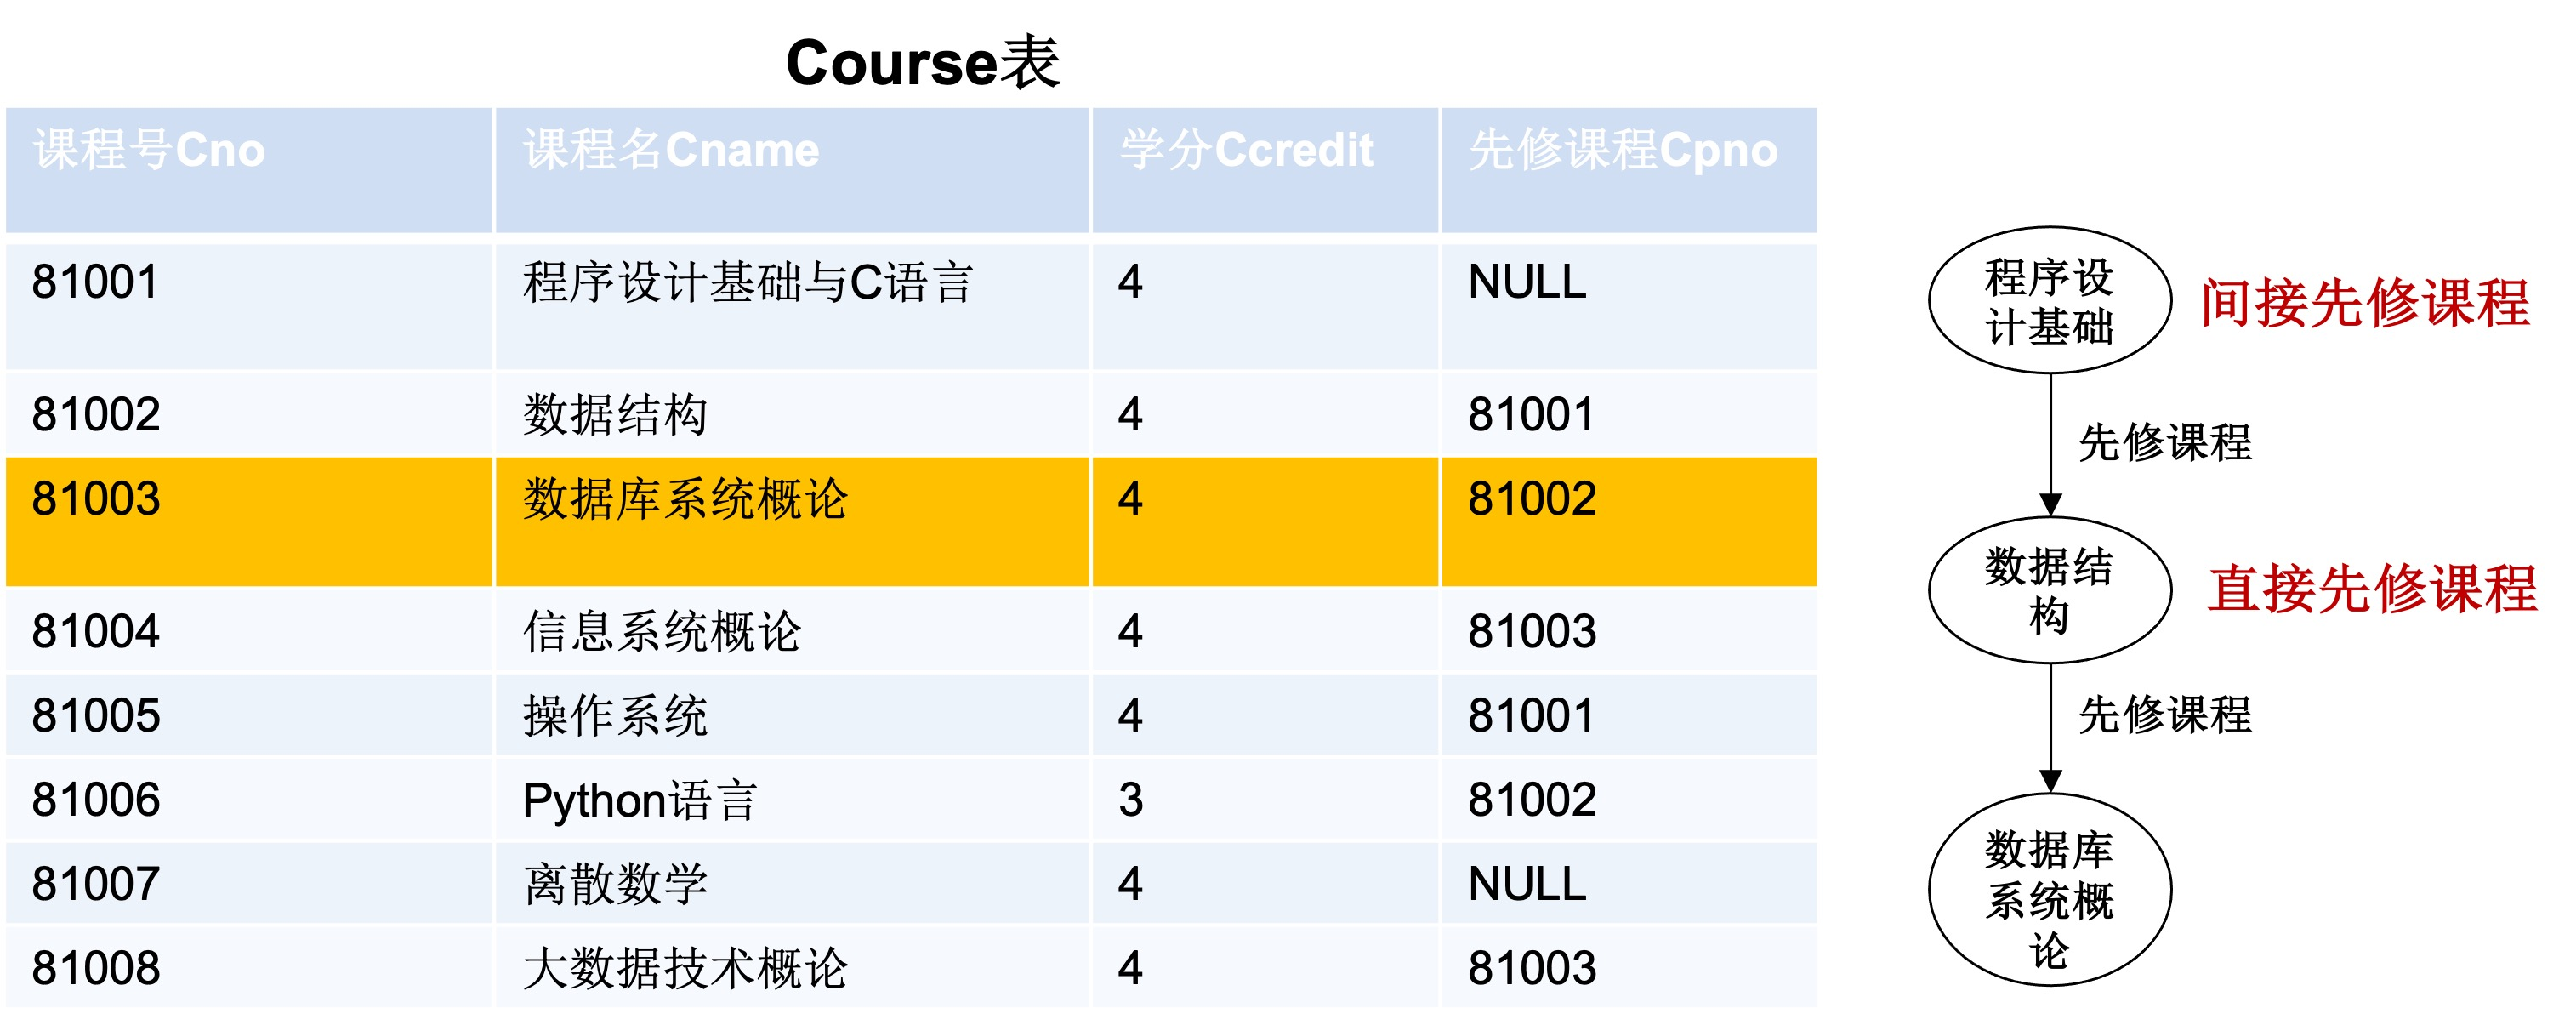
\includegraphics[width=0.8\textwidth]{figure/fig-2.jpg}
    \end{figure}

\framebreak
\item 任务分析:SQL如何表达
    \begin{itemize}
        \item 难点:课程可能同时存在直接先修课和间接先修课
        \item 情况一:如何查询直接先修课:自身连接查询
        \item 情况二:如何查询间接先修课:递归查询\textcolor{red}{(无法表达)}
    \end{itemize}
\end{itemize}
\end{frame}

\begin{frame}[fragile,allowframebreaks]{直接先修课的SQL语句表达}
\begin{itemize}
    \item 如何查询直接先修课:自连接

\begin{enumerate}
    \item 步骤1:找出“数据库系统概论”课程的全部直接先修课:记为L[1];
    如果L[1]为空,则任务一结束
\begin{block}{}
\begin{lstlisting}
SELECT B.Cname 
FROM Course A, Course B
WHERE A.Cname = '数据库系统概论' 
AND A.Cpno=B.Cno;
\end{lstlisting}
\end{block} 
\end{enumerate}
\end{itemize}
\end{frame}

\begin{frame}[fragile,allowframebreaks]{间接先修课的SQL语句表达}
\begin{itemize}
\item 如何查询间接先修课:递归执行

\begin{enumerate}
 \setcounter{enumi}{1}
\item 步骤i (i>=2):找出集合L[i-1]中每一门课程的全部直接先修课,并计算它们的并集,记为L[i]
\item 迭代执行步骤i, 直到并集L[i]为空,输出L[1] $\bigcup \dots \bigcup$ L[i]

\begin{block}{}
\begin{lstlisting}
SELECT B.Cname 
FROM Course A, Course B
WHERE A.Cname = '数据结构' AND A.Cpno=B.Cno;


SELECT B.Cname 
FROM Course A, Course B
WHERE A.Cname = '程序设计基础与C语言' AND A.Cpno=B.Cno;
\end{lstlisting}
\end{block} 

\end{enumerate}


\begin{itemize}
    \item 在第2章图2.1所示的Course 表中,执行步骤1,找出“数据库系统概论”课程的直接先修课“数据结构”,即为L[1]
    \item 执行步骤2,找出“数据结构”课程的先修课“程序设计基础与C语言”,即为L[2]
    \item 步骤3,找出“程序设计基础与C语言”的先修课,得到 L[3]
    \item 可以发现L[3]为空,递归查询结束。根据计算结果L[1]$\bigcup$L[2],任务1的输出如表所示

   \begin{figure}
        \centering
        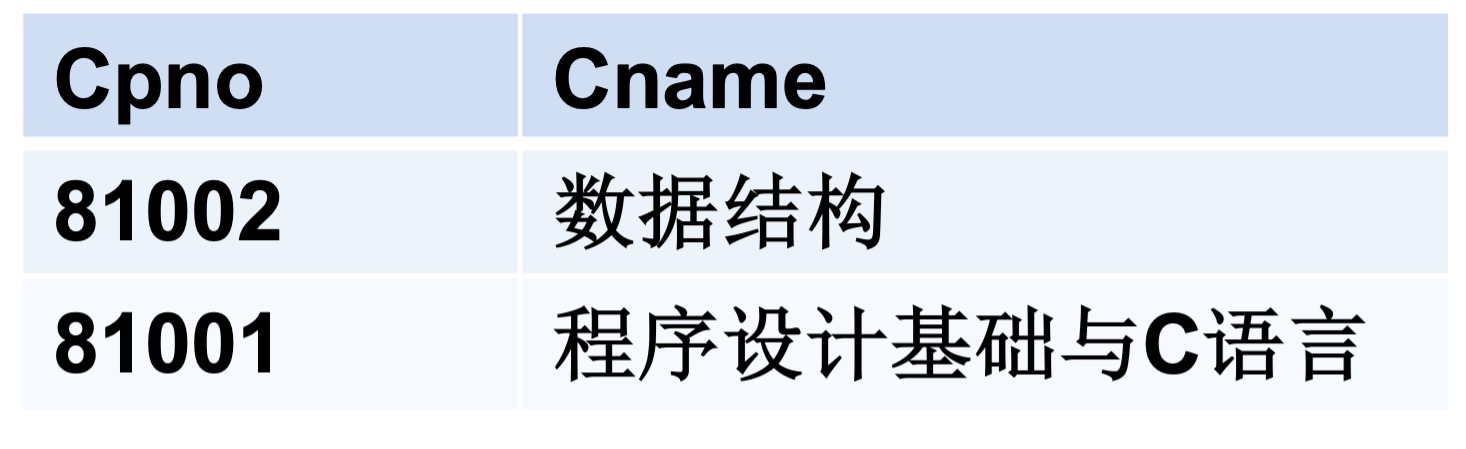
\includegraphics[width=0.5\textwidth]{figure/fig-3.jpg}
    \end{figure}

\end{itemize}

\end{itemize}
\end{frame}




\begin{frame}[allowframebreaks]{【任务2】打印一周内将过生日的学生信息}
\begin{itemize}
    \item 【任务2】打印一周内将过生日的学生信息
   \begin{figure}
        \centering
        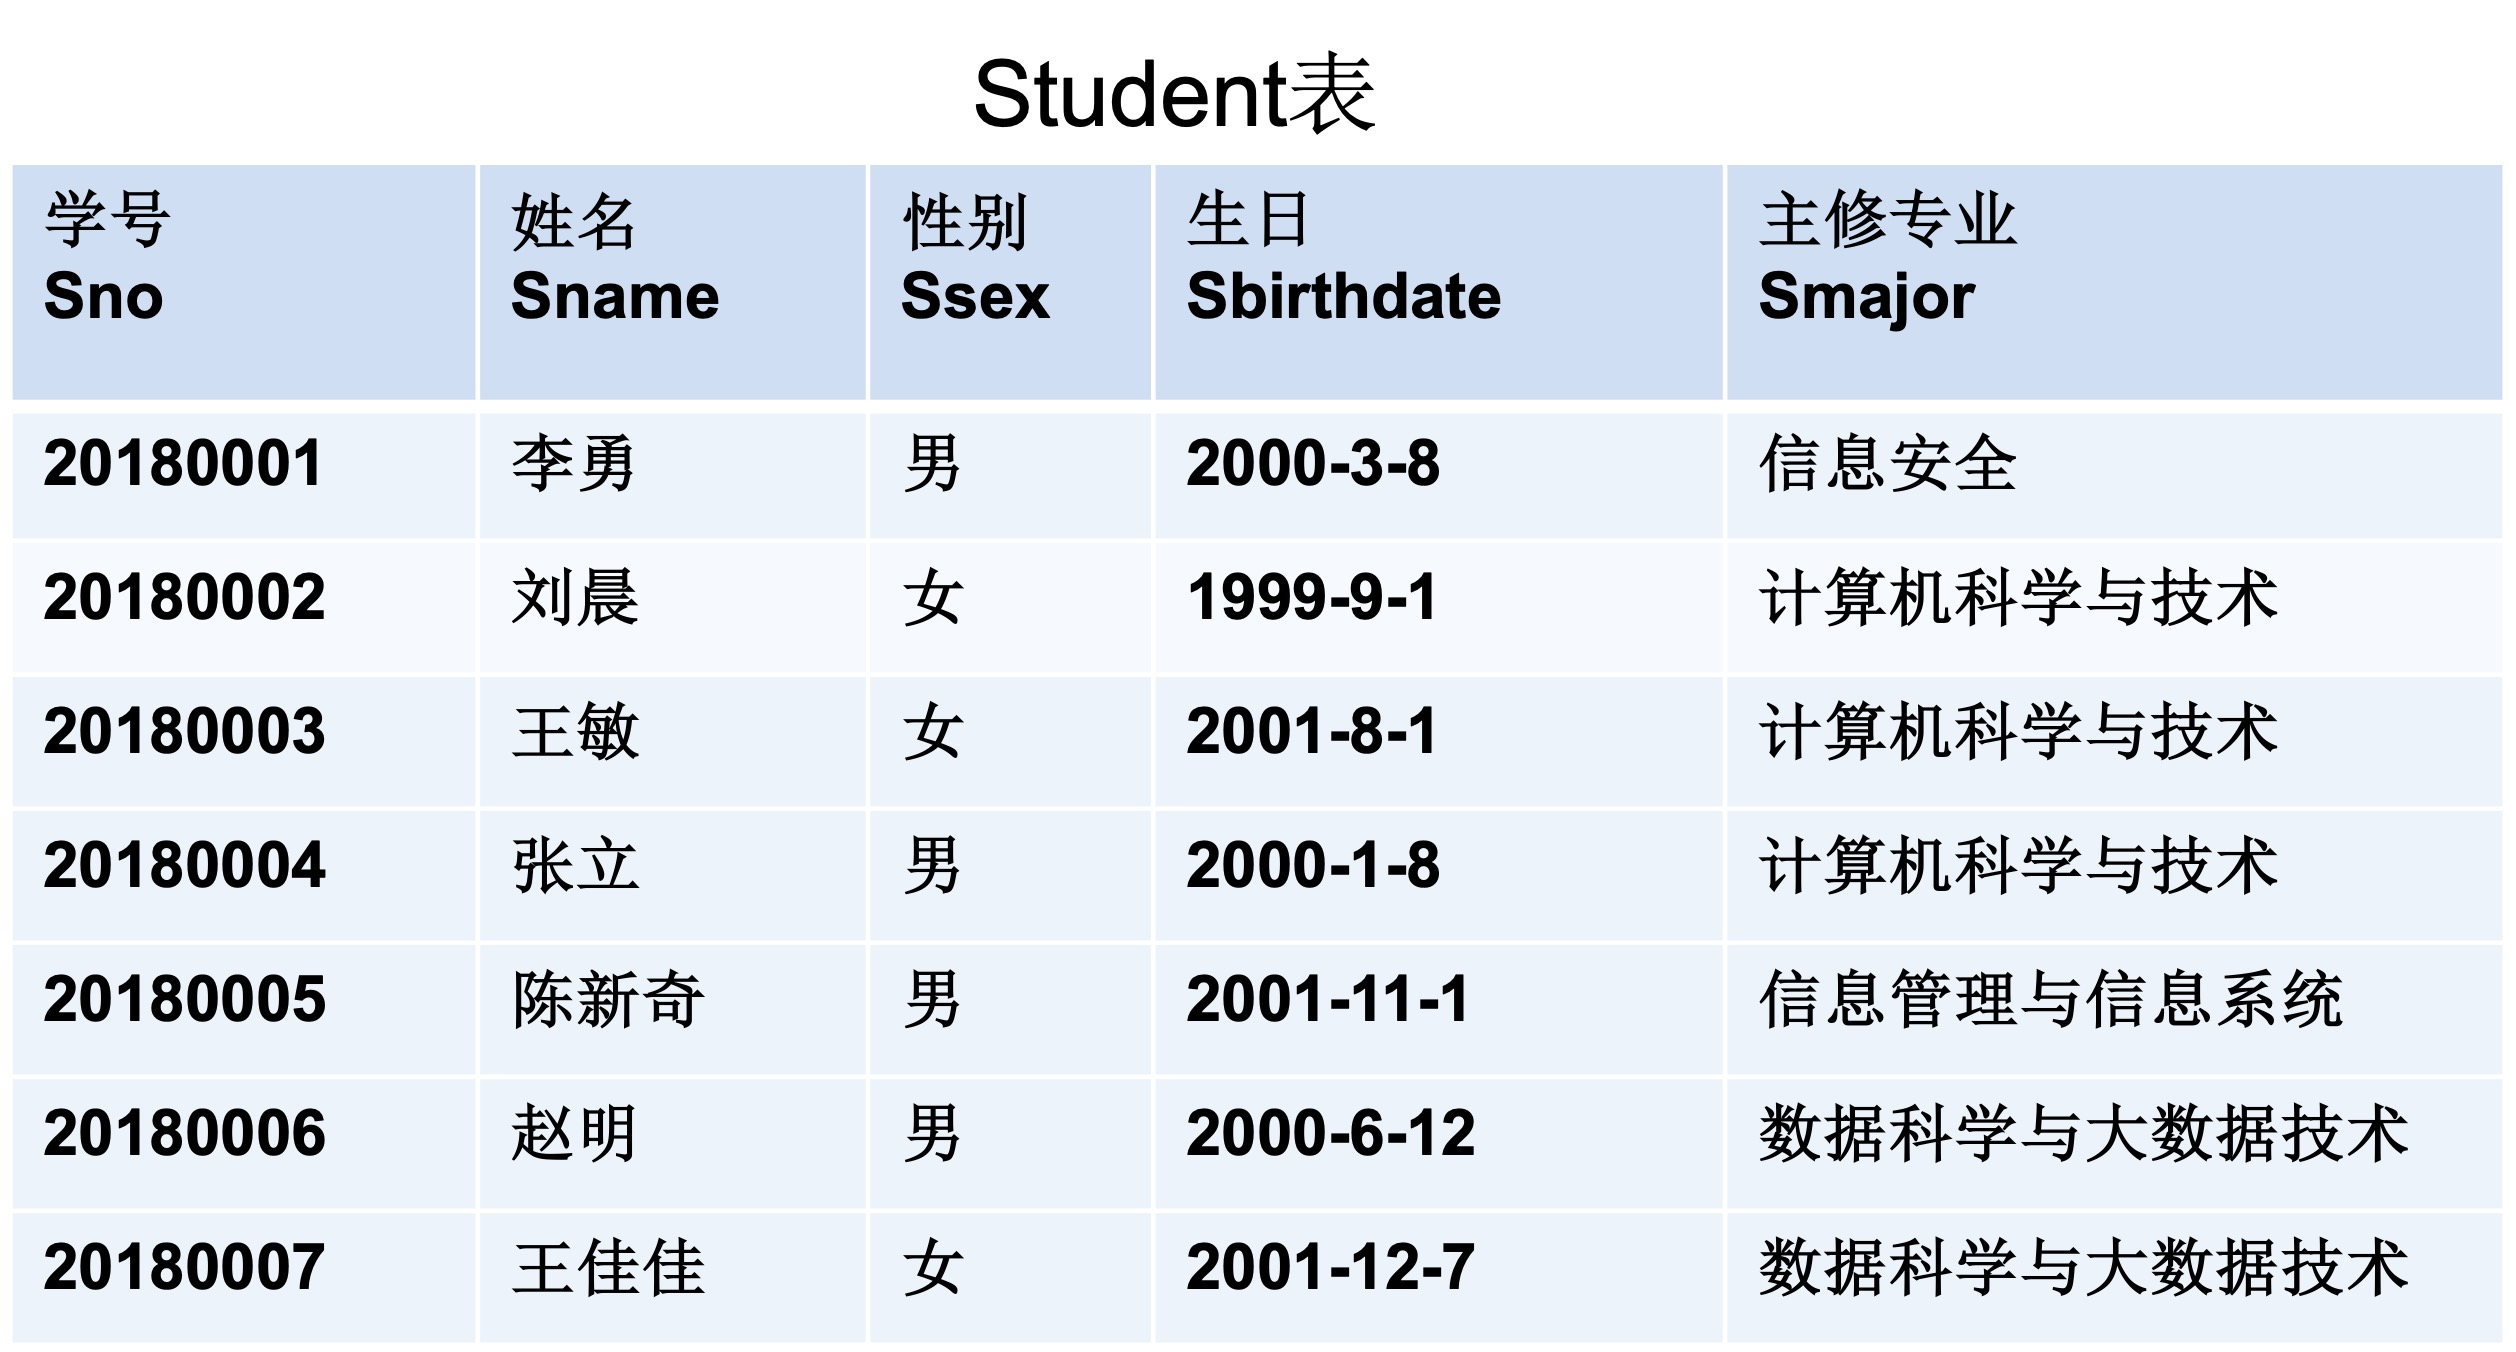
\includegraphics[width=0.7\textwidth]{figure/fig-4.jpg}
    \end{figure}
\end{itemize}

\framebreak
\begin{itemize}
    \item 任务分析:SQL如何表达
\begin{itemize}
    \item 任务2需要数据库系统提供内置函数(本任务主要是日期数)。其求解思路为:扫指个学生的出生日期,例如 2000-6-12,并执行以下步骤
    \begin{enumerate}
\item 把出生日期的年份换成当前日期所在的年份(例如2021),即2021-6-12
\item 获取当前系统的日期,例如 2021-6-9
\item 确定过生日的日期范围[2021-6-9,2021-6-16],即以当前日期为下界,当	前日期后的第七天作为上界
\item 判断出生日期是否在上述日期范围内,如果是,输出该学生信息
    \end{enumerate}
\end{itemize}
\end{itemize}
    
\end{frame}

\begin{frame}[allowframebreaks]{【任务3】计算学生的平均学分绩点GPA}
\begin{itemize}
    \item 【任务3】给定学生学号,计算学生的平均学分绩点GPA
\begin{figure}
    \centering
    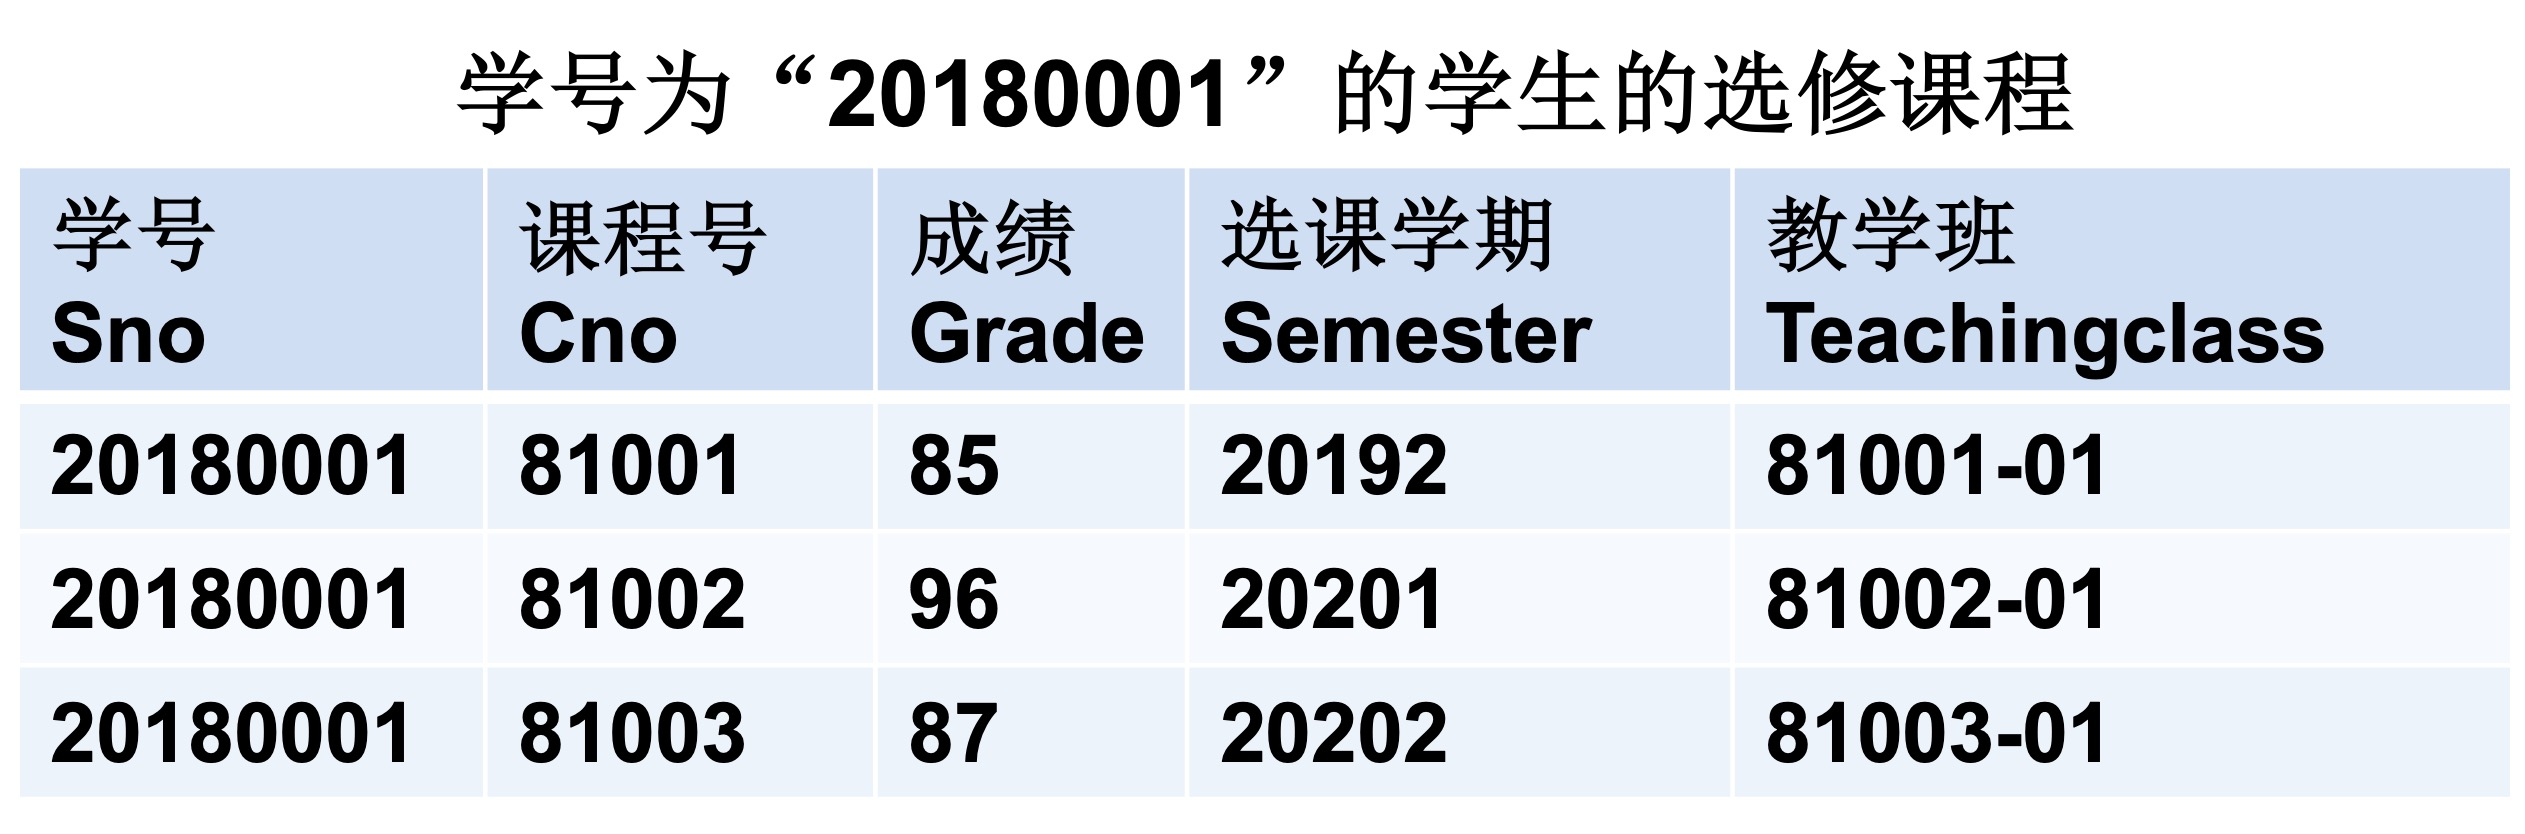
\includegraphics[width=0.8\textwidth]{figure/fig-5.jpg}
\end{figure}

\framebreak
\item 任务分析:SQL如何表达
    \begin{itemize}
    \item 难点:需要用户自主设计业务处理逻辑?
    \item 本任务的求解思路:给定学生学号,找出该学生所有选修课程的学分、成绩;
    \item 根据每门课程的成绩,参照“成绩和绩点对照表”,确定该成绩所处的范围,找出该门课程对应的绩点。
    \end{itemize}
\end{itemize}

\end{frame}

\begin{frame}[allowframebreaks]{【任务4】教学评价浏览与反馈}
\begin{itemize}
    \item 【任务4】教学评价浏览与反馈:学生通过交互界面提交对某一位任课老师的教学评价意见,教师浏览这些评价意见并提供反馈信息
\begin{figure}
    \centering
    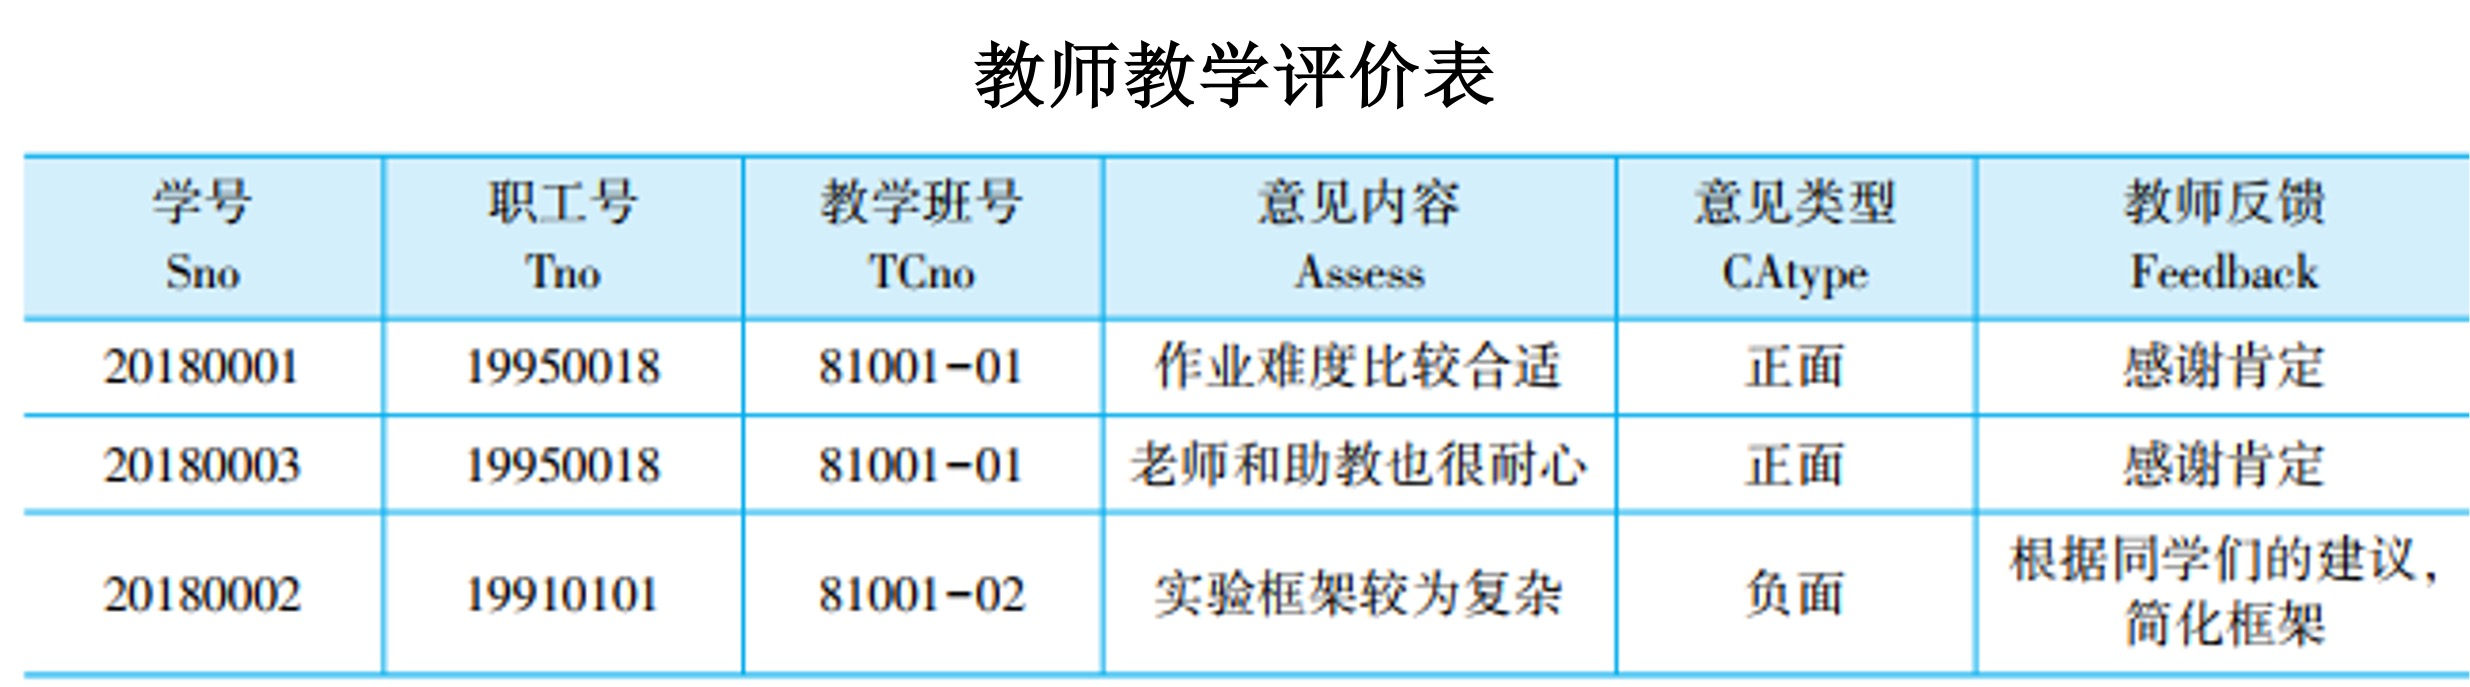
\includegraphics[width=0.8\textwidth]{figure/fig-6.jpg}
\end{figure}
\framebreak
    \item 任务分析:SQL如何表达
\begin{itemize}
    \item 难点:需要建立交互功能
    \item 一方面,学生需要找到指定的教学班和授课教师,建立如图所示的交互界面并输入课程评价。
    \item 另一方面,还要建立如图所示的交互界面,教师浏览教学班学生的评价意见,并针对每条评价逐一做出回复
\begin{figure}
    \centering
    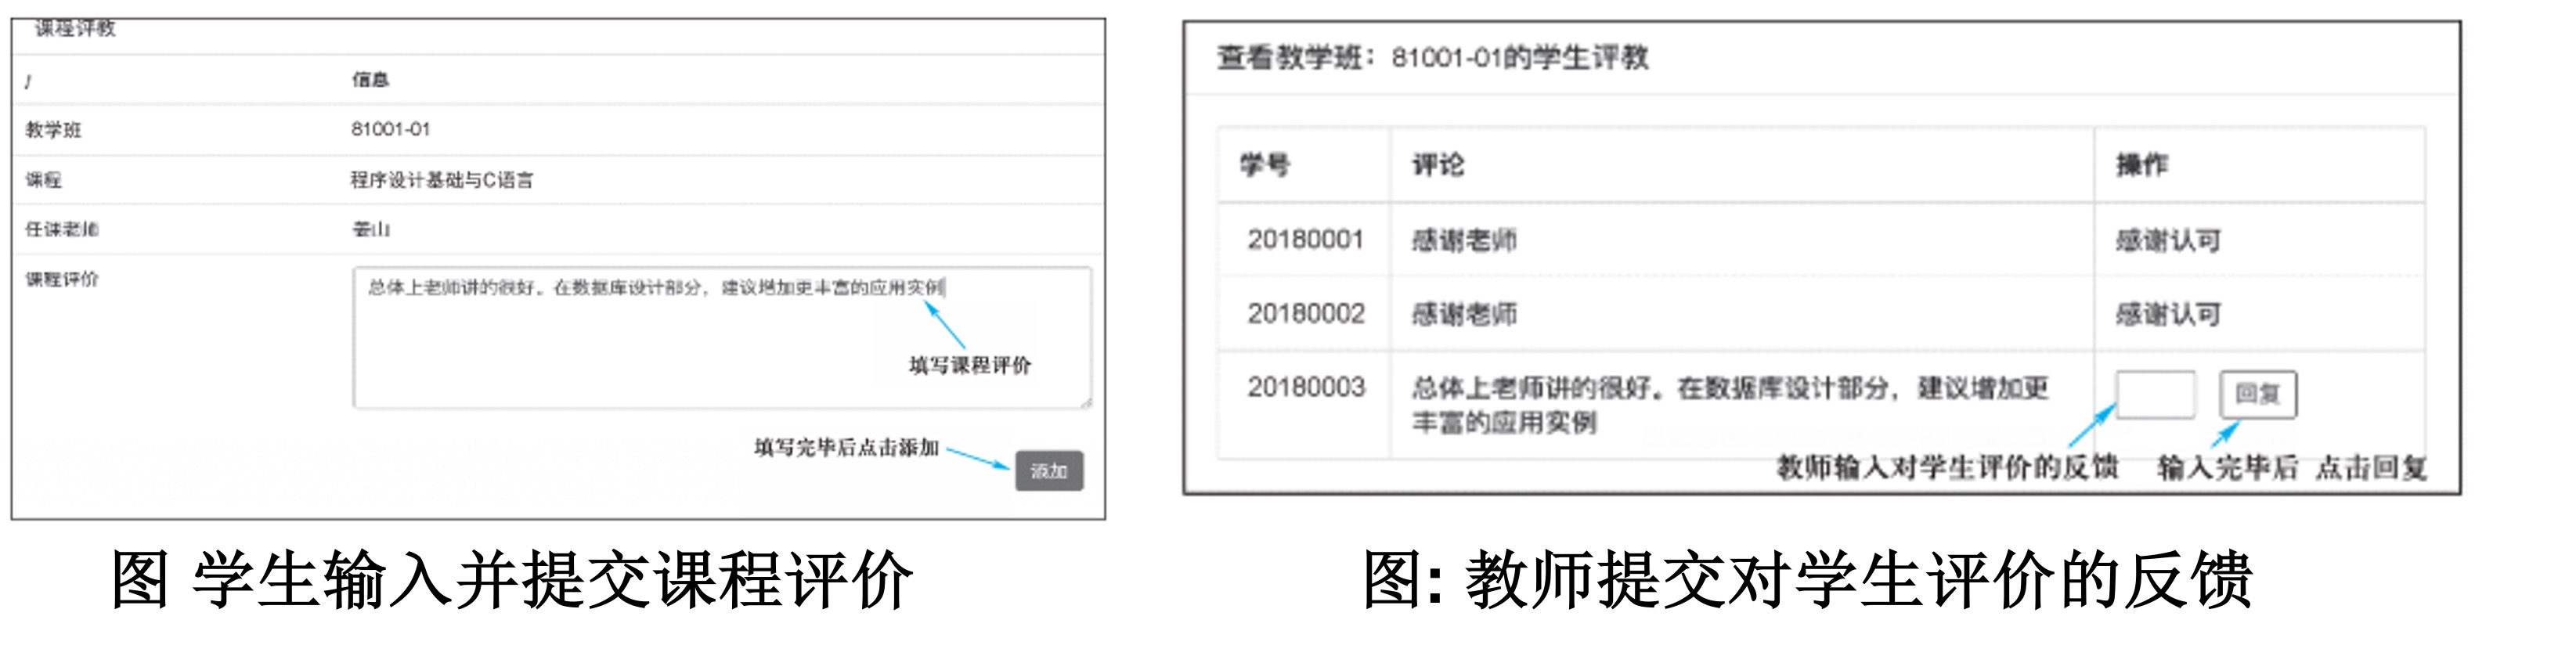
\includegraphics[width=0.8\textwidth]{figure/fig-7.jpg}
\end{figure}

\end{itemize}
\end{itemize}
\end{frame}

\begin{frame}[allowframebreaks]{小结}
\begin{itemize}
    \item SQL语言表达能力的限制
\begin{itemize}
\item 无法表达递归等复杂操作--例如间接先修课的查询
\item 无法对数据进行复杂操作--查询一周内将过生日的同学
\item 无法自主设计业务处理逻辑—计算学生平均学分绩点
\item 无法进行交互式操作--教学评价与反馈
\end{itemize}


\end{itemize}
\end{frame}


\subsection{1.2 扩展SQL的功能}
\begin{frame}[allowframebreaks]{扩展SQL语言的功能}
\begin{itemize}
    \item 1.引入新的SQL子句
    \item 2.引入新的内置函数
    \item 3.引入PL/SQL与存储过程/存储函数
\end{itemize}
\end{frame}

\begin{frame}[allowframebreaks]{引入新的SQL子句}
\begin{itemize}
    \item 以【任务1】为例,SQL标准引入了WITH RECURSIVE子句,可执行递归查询
    \item 类似于WITH RECURSIVE子句的SQL扩展还有很多,例如面向联机分析处理的窗口子句,面向空间数据管理、文档数据管理的SQL语言扩展等
    \item 在介绍WITH RECURSIVE子句之前,先了解WITH子句的用法
\end{itemize}
\end{frame}

\begin{frame}[allowframebreaks,fragile]{WITH子句 格式}
\begin{itemize}
    \item WITH子句的一般格式:
\end{itemize}
    \begin{block}{}
\begin{lstlisting}
WITH RS1[(<目标列>,<目标列>)]AS    /* RS1为临时结果集的命名*/
(SELECT 语句1)[,                  /* RS1对应SELECT 语句的执行结果*/
/*SELECT语句1中的目标列与RS1中的目标列必须保持一致*/
RS2[(<目标列>,<目标列>)]AS        /* RS2为临时结果集的命名*/
(SELECT 语句2),…]                /* RS2对应SELECT 语句的执行结果*/
/*SELECT语句2中的目标列与RS2中的目标列必须保持一致*/
    SQL语句;                      /* 执行与RS1,RS2,…,相关的查询*/
\end{lstlisting}
\end{block} 
\end{frame}

\begin{frame}[allowframebreaks,fragile]{WITH子句 示例}
\begin{itemize}
\item 例: 求81001-01和81001-02两个教学班之间学生选课平均成绩的差异。
\end{itemize}
    \begin{block}{}
\begin{lstlisting}
WITH 
RS1(Grade)
        AS 
        (SELECT AVG(Grade) FROM SC 
        WHERE Teachingclass = '81001-01'),
RS2(Grade)
        AS 
        (SELECT AVG(Grade) FROM SC 
        WHERE Teachingclass = '81001-02')
SELECT RS1.Grade-RS2.Grade FROM RS1,RS2;
\end{lstlisting}
\end{block} 
\end{frame}

\begin{frame}[allowframebreaks,fragile]{WITH RECURSIVE子句 格式}
\begin{itemize}
\item WITH RECURSIVE子句的一般格式:
\end{itemize}

\begin{block}{}
\begin{lstlisting}
WITH RECURSIVE RS AS
    (
        SEED QUERY           /*初始化查询的临时结果集,记为L[1]*/
        UNION [ALL]          /*是否需要保留重复记录,加ALL为保留*/
        RECURSIVE QUERY      
        /*执行递归查询,得到全部临时结果集,即L[2]∪…∪L[i]*/
   ) 
   SQL语句           /*执行与RS相关的查询*/
\end{lstlisting}
\end{block} 

\end{frame}

\begin{frame}[allowframebreaks,fragile]{WITH RECURSIVE子句 示例}
\begin{itemize}
    \item 【任务1】打印“数据库系统概论”课程的所有先修课信息
\end{itemize}
    \begin{figure}
    \centering
    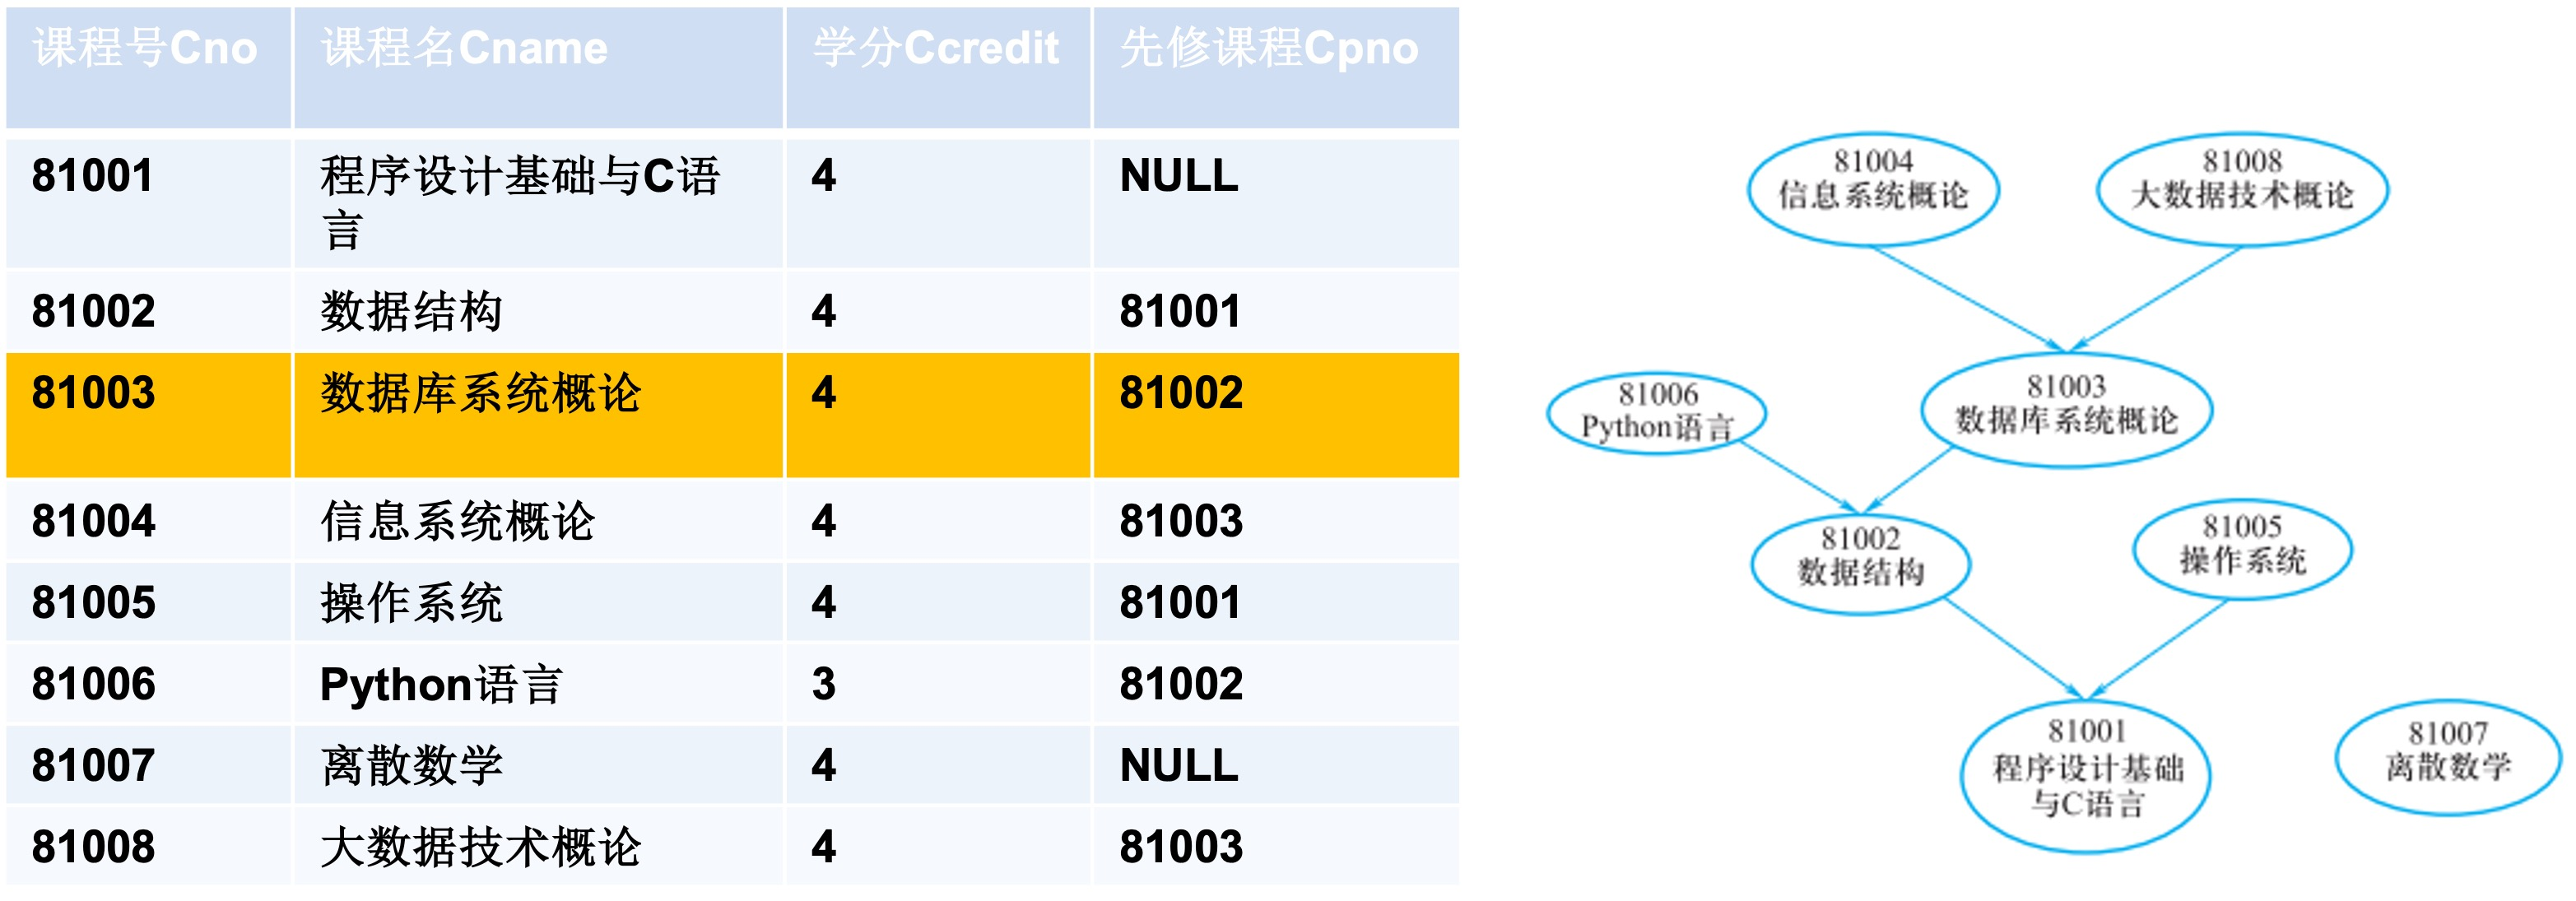
\includegraphics[width=0.9\textwidth]{figure/fig-8.jpg}
\end{figure}

\framebreak
\begin{itemize}
    \item 【任务1】打印“数据库系统概论”课程的所有先修课信息
\end{itemize}

\begin{block}{}
\begin{lstlisting}
WITH RECURSIVE RS AS     
    (SELECT Cpno FROM Course WHERE Cname = '数据库系统概论'
    /*初始化RS,假设结果集为L[1],即“数据库系统概论”的所有直接先修课*/
    UNION  
    SELECT Course.Cpno FROM Course,RS WHERE RS.Cpno = Course.Cno)
    /*递归查询第i层(i>=1)的数据,即第i-1层数据的直接先修课课程号,并更新RS*/
SELECT Cno, Cname FROM Course WHERE Cno IN (SELECT Cpno FROM RS);
/*根据RS中记录的所有先修课程号,通过查找课程表,输出课程号与课程名*/

\end{lstlisting}
\end{block} 
\end{frame}


\begin{frame}{引入新的内置函数}
    \begin{itemize}
        \item SQL常用的内置函数可以分为:
\begin{itemize}
    \item 数学函数(如绝对值函数等)
    \item 聚合函数(如求和、求平均函数等)
    \item 字符串函数(如求字符串长度、求子串函数等)
    \item 日期和时间函数(如返回当前日期函数等)
    \item 格式化函数(如字符串转IP地址函数等)
    \item 控制流函数(如逻辑判断函数等)
    \item 加密函数(如使用密钥对字符串加密函数等)
    \item 系统信息函数(如返回当前数据库名、服务器版本函数等)
\end{itemize}
    \end{itemize}
\end{frame}

\begin{frame}[allowframebreaks,fragile]{日期和时间函数 示例}
    \begin{itemize}
        \item 【任务2】打印一周内将过生日的学生信息
    \end{itemize}

\begin{block}{}
\begin{lstlisting}
SELECT Sno, Sname, Ssex, Sbirthdate, Smajor 
FROM Student 
WHERE to_date(to_char(current_date,'yyyy') || '-' || to_char(Sbirthdate,'mm-dd')) 
BETWEEN CURRENT_DATE AND CURRENT_DATE + INTERVAL '7' DAY;
\end{lstlisting}
\end{block} 
\begin{itemize}
    \item 在WHERE 语句中使用了以下内置函数:
    \begin{enumerate}
        \item 内置函数 \lstinline{current_date} 返回当前的系统日期,例如 2021-6-9
        \item 内置函数 \lstinline{to_char(current_data,'yyyy')}返回当前系统日期的年份,例如 2021; \lstinline{to_char(Sbirthdate,'mm-dd')}返回学生出生日期中具体的月份和日期,例如 6-9
        \item \lstinline{to_date(to_char(current_date,'yyyy')||'-'|| to_char(Sbirthdate,'mm-dd'))}表示把当前年份与出生日期用'-'连在一起。符号\lstinline{'‖'}用于把其左右两边的字符串连在一起
        \item 内置函数 \lstinline{to_date()}的作用是将字符类型按一定格式转化为日期类型。
        \item \lstinline{CURRENT_DATE + INTERVAL '7' DAY}是对当前的日期调整后的日期。参数interval是年(yyyy)、季度(q)、月(m)、日(d)、时(h)等粒度的时间单位。例如,\lstinline{CURRENT_DATE + INTERVAL '7' DAY}获得当前日期之后第七天的日期,即返回2021-6-16
    \end{enumerate}
    \item 通过执行此WHERE语句,判断学生表中每位学生转换后的出生日期是否在[2021-6-9,2021-6-16]区间内,如果是,打印该学生的信息
\end{itemize}
\end{frame}

\begin{frame}{引入PL/SQL与存储过程/存储函数}
    \begin{itemize}
        \item 关系数据库管理系统中引入PL/SQL、存储过程和自定义函数等方法,使得用户可以自定义程序逻辑,开发完成业务逻辑复杂的应用系统。
    \end{itemize}
\end{frame}

\subsection{1.3 通过高级语言实现复杂应用}

\begin{frame}{通过高级语言实现复杂应用}
    \begin{itemize}
        \item 通过动态链接库调用的方式
        \begin{itemize}
            \item 关系数据库管理系统的功能被包装成一个子程序,由应用程序通过动态链接库调用来获得数据管理的功能
        \end{itemize}
        \item 基于嵌入式SQL的方式
        \begin{itemize}
            \item 将SQL嵌入到高级语言中混合编程,SQL语句负责操纵数据库,高级语言语句负责控制逻辑流程
        \end{itemize}
        \item 基于ODBC/JDBC的中间件方式
        \begin{itemize}
            \item 建立了连接不同数据库的一组规范。无论使用什么数据库,都采用同样的一组API来访问数据库
        \end{itemize}
    \end{itemize}
\end{frame}









\section{过程化SQL}
\subsection{2.1 过程化SQL的块结构}
\begin{frame}[allowframebreaks,fragile]{2.1 过程化SQL的块结构}
    \begin{itemize}
        \item 过程化SQL 
        \begin{itemize} 
            \item SQL的扩展
            \item 增加了过程化语句功能
            \item 基本结构是块
            \begin{itemize} 
                \item 块之间可以互相嵌套
                \item 每个块完成一个逻辑操作
            \end{itemize}
        \end{itemize}
        \item 过程化SQL块的基本结构
        \begin{enumerate}
            \item 定义部分: DECLARE 变量、常量、游标、异常等   
            \begin{itemize}
                \item 定义的变量、常量等只能在该基本块中使用
                \item 当基本块执行结束时,定义就不再存在
            \end{itemize}
            \item 执行部分
\begin{block}{}
\begin{lstlisting}
BEGIN
    SQL语句、过程化SQL的流程控制语句
    EXCEPTION
    异常处理部分
END;
\end{lstlisting}
\end{block} 
\begin{itemize}
    \item 遇到不能继续执行的情况称为异常
    \item 在出现异常时,采取措施来纠正错误或报告错误
\end{itemize}
        \end{enumerate}
    \end{itemize}
\end{frame}

\subsection{变量和常量的定义}
\begin{frame}[allowframebreaks,fragile]{2.2 变量和常量的定义}
\begin{enumerate}
    \item 变量和常量的定义
    \begin{itemize}
        \item 变量名 数据类型 \lstinline{[[NOT NULL]:=初值表达式]}
        \item 变量名 数据类型 \lstinline{[[NOT NULL] 初值表达式]}
    \end{itemize}
    \item 常量定义
    \begin{itemize}
        \item 常量名 数据类型 \lstinline{CONSTANT :=常量表达式}
        \item 常量必须要赋予一个值,并且该值在存在期间或常量的作用域内不能改变。如果试图修改它,过程化SQL将返回一个异常
    \end{itemize}
    \item 赋值语句
    \begin{itemize}
    \item \lstinline{变量名称 :=表达式}
    \end{itemize}
\end{enumerate}
\end{frame}



\subsection{流程控制}
\begin{frame}[allowframebreaks,fragile]{2.3 流程控制}
\begin{itemize}
    \item 过程化SQL功能
    \begin{enumerate}
        \item 条件控制语句: IF-THEN,IF-THEN-ELSE和嵌套的IF语句 
        \begin{itemize}
            \item IF-THEN语句格式
            \item IF-THEN-ELSE语句格式
            \item 在THEN和ELSE子句中还可以再包含IF语句,即IF语句可以嵌套
        \end{itemize}
\begin{block}{}
\begin{lstlisting}
IF condition THEN
   Sequence_of_statements;        
END IF;   

IF condition THEN
   Sequence_of_statements1;  
ELSE
   Sequence_of_statements2;  
END IF;
\end{lstlisting}
\end{block} 
        
        \framebreak
        
        \item 循环控制语句: LOOP, WHILE-LOOP, FOR-LOOP

\begin{block}{}
\begin{lstlisting}
LOOP
  Sequence_of_statements;        
END LOOP;
\end{lstlisting}
\end{block} 
        \begin{itemize}
            \item 多数数据库服务器的过程化SQL都提供EXIT、BREAK或LEAVE等循环结束语句,保证LOOP语句块能够在适当的条件下提前结束
        \end{itemize}
\framebreak
\begin{block}{}
\begin{lstlisting}
WHILE condition LOOP
    Sequence_of_statements;
END LOOP;

\end{lstlisting}
\end{block} 

        \begin{itemize}
            \item 每次执行循环体语句之前,首先对条件进行求值
            \item 如果条件为真,则执行循环体内的语句序列
            \item 如果条件为假,则跳过循环并把控制传递给下一个语句
        \end{itemize}
\framebreak
\begin{block}{}
\begin{lstlisting}
FOR count IN [REVERSE] bound1 … bound2 LOOP
    Sequence_of_statements;
END LOOP;
\end{lstlisting}
\end{block} 

        \framebreak
        \item 错误处理 
        \begin{itemize}
            \item 如果过程化SQL在执行时出现异常,则应该让程序在产生异常的语句处停下来,根据异常的类型去执行异常处理语句 
            \item SQL标准对数据库服务器提供什么样的异常处理做出了建议,要求过程化SQL管理器提供完善的异常处理机制 
        \end{itemize}
    \end{enumerate}
\end{itemize}
\end{frame}



\subsection{游标的定义与使用}

\begin{frame}[allowframebreaks,fragile]{2.4 游标的定义与使用}
\begin{itemize}
    \item 游标
    \begin{itemize}
        \item 在过程化SQL中,如果\lstinline{SELECT}语句只返回一条记录,可以将该结果存放到变量中
        \item 当查询返回多条记录时,就要使用游标对结果集进行处理。一个游标与一个SQL语句相关联
        \item 游标的用户接口: 
        
        1.声明游标 2.打开游标 3.使用游标 4.关闭游标
    \end{itemize}    
        \framebreak
    \begin{enumerate}
        \item 声明游标
\begin{block}{}
\begin{lstlisting}
DECLARE 游标名 [(参数1 数据类型, 参数2 数据类型, …)] 
CURSOR FOR 
SELECT语句;
\end{lstlisting}
\end{block} 
        \begin{itemize}
            \item 定义游标仅仅是一条说明性语句,这时关系数据库管理系统并不执行\lstinline{SELECT}语句
        \end{itemize}
\framebreak
        
\item 打开游标
        
\begin{block}{}
\begin{lstlisting}
OPEN 游标名[(参数1 数据类型, 参数2 数据类型, …)];
\end{lstlisting}
\end{block} 
        \begin{itemize}
            \item 打开游标实际上是执行相应的\lstinline{SELECT}语句,把查询结果取到缓冲区中。这时游标处于活动状态,指针指向查询结果集中的第一条记录
        \end{itemize}
        \framebreak
\item 使用游标

\begin{block}{}
\begin{lstlisting}
FETCH 游标名 INTO 变量1[, 变量2,…];
\end{lstlisting}
\end{block} 
\begin{itemize}
    \item 变量必须与\lstinline{SELECT}语句中的目标列表达式一一对应
    \item 用FETCH语句把游标指针向前推进一条记录,同时将缓冲区中的当前记录取出来送至变量供过程化SQL进一步处理
    \item 循环执行FETCH语句,逐条取出结果集中的行进行处理
\end{itemize}

        \framebreak

\item 关闭游标
\begin{block}{}
\begin{lstlisting}
CLOSE 游标名;
\end{lstlisting}
\end{block} 
\begin{itemize}
    \item 游标被关闭后就不再和原来的查询结果集相联系
    \item 但被关闭的游标可以再次被打开,与新的查询结果相联系
\end{itemize}





    \end{enumerate}
\end{itemize}
\end{frame}
 
\begin{frame}[fragile]{2.4 游标的定义和使用(例)}
\begin{itemize}
    \item 根据给定学号20180001,使用游标输出该学生的全部选课记录
\begin{block}{}
\begin{lstlisting}[xleftmargin=0.1\textwidth,linewidth=\textwidth]
DECLARE
    CnoOfStudent CHAR(10);
    GradeOfStudent INT;
    mycursor CURSOR FOR 
    SELECT Cno,Grade FROM SC WHERE Sno = '20180001';
BEGIN
    OPEN mycursor;      /*打开游标*/
    LOOP                /*循环遍历游标*/ 
        FETCH mycursor INTO CnoOfStudent, GradeOfStudent; /*检索游标*/
        EXIT WHEN mycursor \%NOTFOUND;
        RAISE NOTICE 'Sno:20180001, Cno:\%, Grade:\%', CnoOfStudent, GradeOfStudent;
    END LOOP;
    CLOSE mycursor;     /*关闭游标*/
END;
\end{lstlisting}
\end{block} 
\end{itemize}
\end{frame}


\subsection{存储过程}
\begin{frame}[allowframebreaks,fragile]{存储过程}
\begin{itemize}
    \item 存储过程
    \begin{itemize}
        \item 类似于高级语言程序,过程化SQL程序也可以被命名和编译,并保存在数据库中,称为存储过程(stored procedure)或存储函数(stored function),供其他过程化SQL调用
        \item 存储过程或存储函数也是一类数据库的对象,需要有创建、删除等语句。这里的存储函数指自定义函数
    \end{itemize}
    \item 存储过程的用户接口
    \begin{enumerate}
        \item 创建存储过程
        \item 执行存储过程 
        \item 修改存储过程
        \item 删除存储过程 
    \end{enumerate}
\end{itemize}
\end{frame}

\begin{frame}[allowframebreaks,fragile]{存储过程-创建存储过程}
\begin{enumerate}
    \item 创建存储过程
\begin{block}{}
\begin{lstlisting}[linewidth=\textwidth]
CREATE OR REPLACE PROCEDURE过程名(
    [[IN|OUT|INOUT] 参数1 数据类型,
    [IN|OUT|INOUT] 参数2 数据类型,
    …]
)                       /*存储过程首部*/ 
AS <过程化SQL块>;       /*存储过程体,描述该存储过程的操作*/
\end{lstlisting}
\end{block} 
\begin{itemize}
    \item 过程名:数据库服务器合法的对象标识
    \item 参数列表:存储过程提供了 IN、OUT、INOUT 三种参数模式,分别对应输入、输出、输入输出三种语义,不声明参数模式时,缺省为 IN 类型。输入参数在被调用时需要指定参数值,输出参数调用时不传入参数值,而是作为返回值返回。输入输出参数调用时需要传入初始值,并会返回操作后的最终值。参数列表中需要指定参数模式、参数名、以及参数的数据类型
    \item 过程体:是一个<过程化SQL块>,包括声明部分和可执行语句部分 
\end{itemize}
\end{enumerate}
\framebreak
\end{frame}

\begin{frame}[fragile]{存储过程-创建存储过程}
\begin{itemize}
    \item 给定学生学号,计算学生的平均学分绩点GPA
    \item 求解思路
    \begin{itemize}
        \item 给定学生学号,找出该学生所有选修课程的学分、成绩
        \item 根据每门课程的成绩,参照成绩和绩点对照表,确定该成绩所处的范围,找出该门课程对应的学分绩点
    \end{itemize}
       \begin{figure}
        \centering
        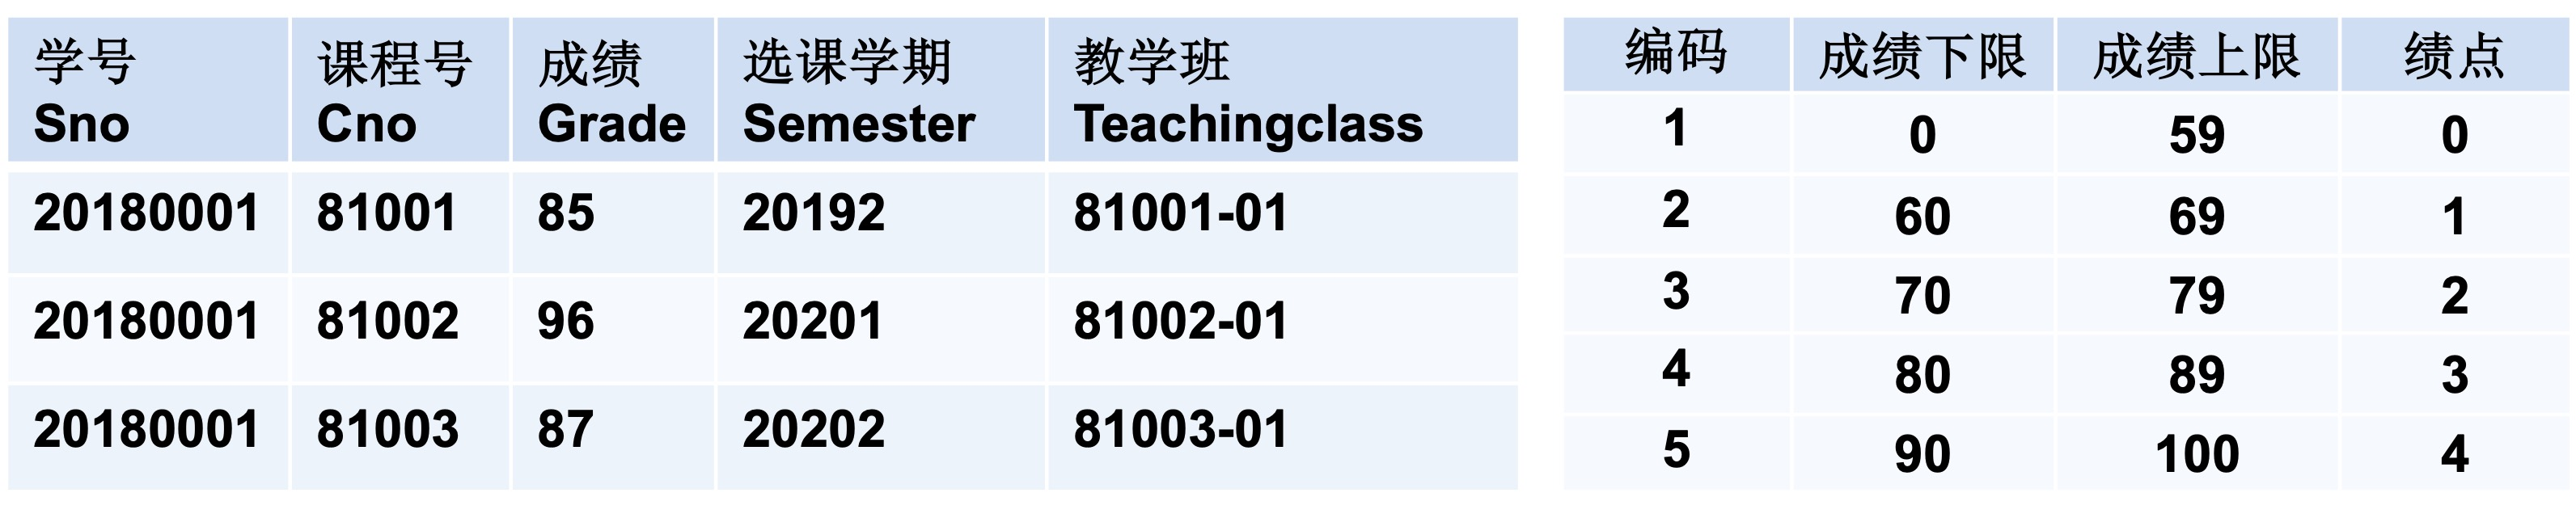
\includegraphics[width=0.8\textwidth]{figure/fig-9.jpg}
    \end{figure}

\end{itemize}
\end{frame}

\begin{frame}[fragile]{存储过程-创建存储过程}
\begin{itemize}
    \item 给定学生学号,计算学生的平均学分绩点GPA
    \item 求解思路
    \begin{itemize}
        \item “81001”课程考试成绩为85分,参照右下表,85分对应成绩范围为[80,89],该门课程对应的学分绩点为3。类似地,课程号为“81002”对应的学分绩点为4, 课程号为“81003”对应的学分绩点为3
        \item 81001-81003三门课程的学分都是4。根据平均学分绩点GPA的计算公式=总学分绩/总学分=(每门课程的学分*对应课程的绩点)的总和/12 = (3*4 + 4*4 + 3*4)/12 = 3.33	
    \end{itemize}
       \begin{figure}
        \centering
        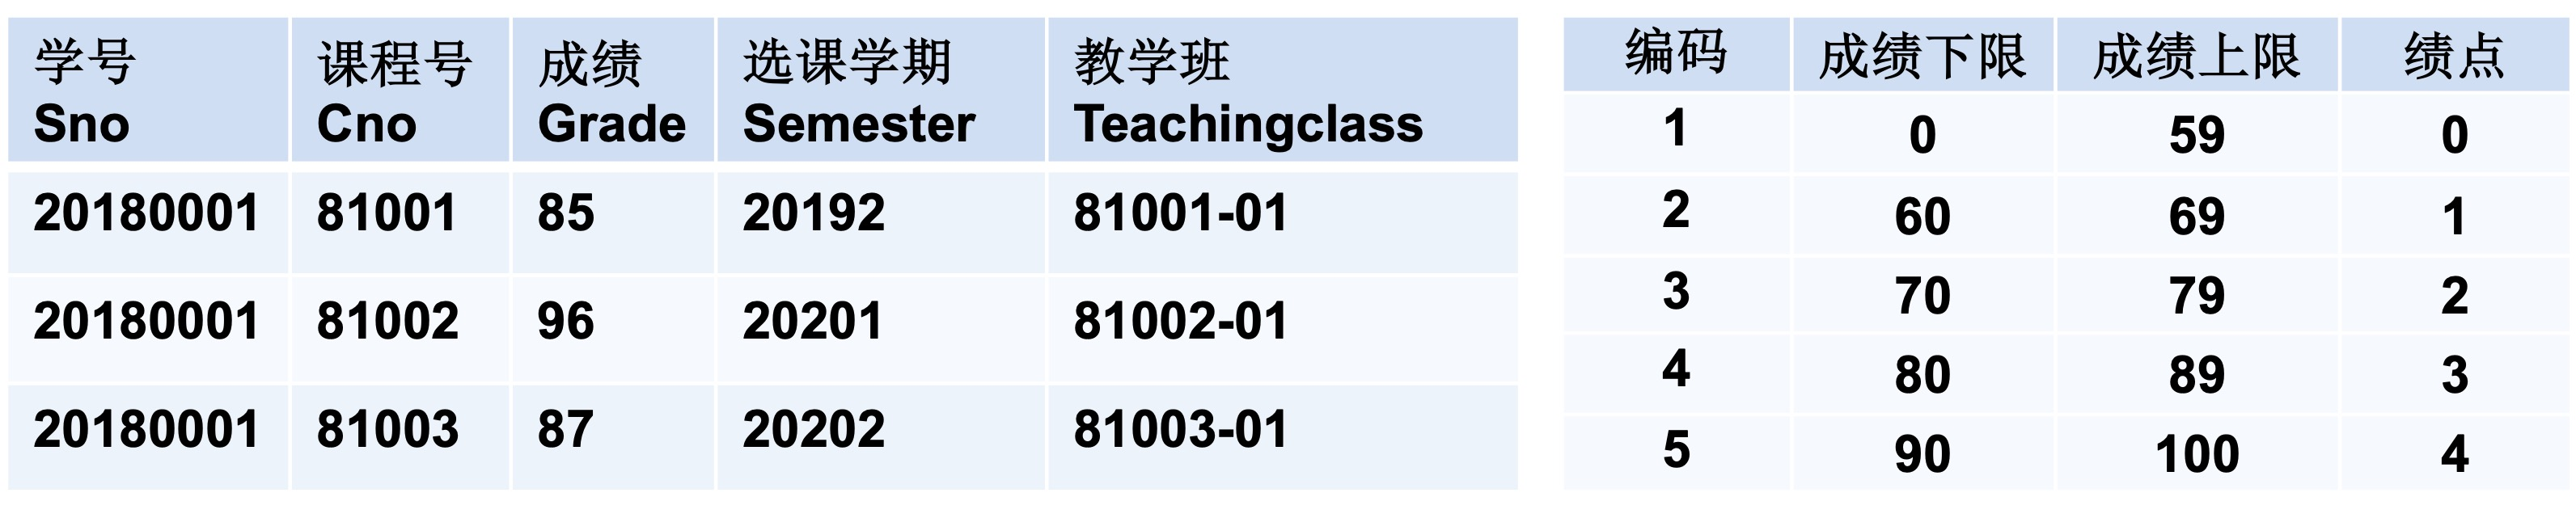
\includegraphics[width=0.8\textwidth]{figure/fig-9.jpg}
    \end{figure}
\end{itemize}
\end{frame}

\begin{frame}[fragile,allowframebreaks]{存储过程-创建存储过程}
\begin{itemize}
    \item 给定学生学号,计算学生的平均学分绩点GPA
\end{itemize}
\begin{block}{}
\begin{lstlisting}[linewidth=\textwidth]
CREATE OR REPLACE PROCEDURE compGPA(      /*定义存储过compGPA*/
    IN inSno CHAR(10),     /*输入参数:学生学号inSno*/
    OUT outGPA FLOAT)      /*输出参数:平均学分绩outGPA*/
    AS 
    DECLARE
        courseGPA INT;     /*声明变量courseGPA,临时存储课程学分绩 */
        totalGPA INT;      /*声明变量totalGPA,临时存储总学分绩 */
        totalCredit INT;   /*声明变量totalCredit,临时存储总学分*/
        grade INT;         /*声明变量grade,临时存储学生成绩 */
        credit INT;         /*声明变量credit ,临时存储课程学分 */
        mycursor CURSOR FOR         /*声明游标mycursor */ 
        SELECT Ccredit, grade FROM SC, Course 
        WHERE Sno = inSno AND SC.Cno = Course.Cno;   
\end{lstlisting}
\end{block}
\framebreak
\begin{block}{}
\begin{lstlisting}[firstnumber=15,linewidth=\textwidth]
    BEGIN 
        totalGPA := 0;
        totalCredit := 0;
        OPEN mycursor;             /*打开游标mycursor */
        LOOP                             /*循环遍历游标*/
            FETCH mycursor INTO credit, grade;     /*检索游标*/
            EXIT WHEN mycursor%NOTFOUND;
            IF grade BETWEEN 90 AND 100 THEN courseGPA := 4.0; 
            ELSIF grade BETWEEN 80 AND 89 THEN courseGPA := 3.0; 
            ELSIF grade BETWEEN 70 AND 72 THEN courseGPA := 2.0; 
            ELSIF grade BETWEEN 60 AND 69 THEN courseGPA := 1.0; 
            ELSE courseGPA := 0; 
            END IF;   /*参照表8.2,根据成绩找出某门课程对应的学分绩点*/
                    totalGPA := totalGPA + courseGPA * credit;
            totalCredit := totalCredit + credit;
        END LOOP;
        CLOSE mycursor;            /*关闭游标mycursor */
        outGPA:= 1.0 * totalGPA / totalCredit;
    END;
\end{lstlisting}
\end{block}

\end{frame}


\begin{frame}[allowframebreaks,fragile]{存储过程}
\begin{enumerate}
\setcounter{enumi}{1}
    \item 执行存储过程

\begin{block}{}
\begin{lstlisting}    
CALL/PERFORM  [PROCEDURE] 过程名([参数1,参数2,...]);
\end{lstlisting}
\end{block}
\begin{itemize}
    \item 使用CALL或者PERFORM等方式激活存储过程的执行
    \item 在过程化SQL中,数据库服务器支持在过程体中调用其他存储过程
\end{itemize}
\end{enumerate}

\framebreak
\begin{itemize}
    \item 查询学号为“20180001”学生的课程GPA。
    \begin{itemize}
        \item 在调用含有输入参数和输入输出参数的存储过程时,需要指定具体的参数值。在调用含有输出参数的存储过程时,对应位置不需要传入参数值,但需要事先定义输出变量
    \end{itemize}
\end{itemize}

\begin{block}{}
\begin{lstlisting}
DECLARE outGPA FLOAT;
BEGIN
    CALL compGPA('20180001',outGPA);
    RAISE NOTICE 'GPA: %', outGPA;
END;

\end{lstlisting}
\end{block}

\end{frame}

\begin{frame}[allowframebreaks,fragile]{存储过程}
\begin{enumerate}
\setcounter{enumi}{2}
    \item 修改存储过程
    \begin{itemize}
        \item 重命名/重新编译
\begin{block}{}
\begin{lstlisting}
ALTER PROCEDURE 过程名1  RENAME TO 过程名2;
ALTER PROCEDURE 过程名1 COMPILE;
\end{lstlisting}
\end{block}
    \end{itemize}
    \item 删除存储过程 
\begin{block}{}
\begin{lstlisting}
DROP  PROCEDURE 过程名;
\end{lstlisting}
\end{block}

\end{enumerate}
\end{frame}


\begin{frame}[allowframebreaks,fragile]{存储过程}
\begin{itemize}
    \item 存储过程的优点
    \begin{enumerate}
\item 运行效率高
\item 降低了客户机和服务器之间的通信量	
\item 方便实施企业规则
\end{enumerate}
\end{itemize}
\end{frame}

\subsection{存储函数}
\begin{frame}[allowframebreaks,fragile]{存储函数}
\begin{itemize}
    \item 存储函数和存储过程的异同
    \begin{enumerate}
\item 同: 都是持久性存储模块
\item 异:函数必须指定返回的类型
\end{enumerate}
\end{itemize}
\end{frame}

\begin{frame}[allowframebreaks,fragile]{存储函数}
\begin{enumerate}
    \item 函数的定义/执行/修改语句 
\begin{block}{}
\begin{lstlisting}
CREATE OR REPLACE FUNCTION 函数名([参数1 数据类型, 参数2数据类型, ...]) 
RETURNS <类型>
AS  <过程化SQL块>;

CALL/SELECT 函数名 ([参数1,参数2,…]);

ALTER FUNCTION 函数名1 RENAME TO 函数名2;
ALTER FUNCTION 函数名 COMPILE;

\end{lstlisting}
\end{block}

\end{enumerate}

\end{frame}





\section{JDBC编程}
\subsection{JDBC工作原理概述}
\begin{frame}[allowframebreaks,fragile]{JDBC工作原理概述}
\begin{itemize}
    \item JDBC (\textbf{J}ava \textbf{D}ata\textbf{B}ase \textbf{C}onnection)
    \begin{itemize}
        \item 由于不同的数据库管理系统的存在,在某个关系数据库管理系统下编写的应用程序就不能在另一个关系数据库管理系统下运行  
        \item 许多应用程序需要共享多个部门的数据资源,访问不同的关系数据库管理系统
    \end{itemize}
    \item JDBC 是面向Java 语言的软件开发工具包(Java Development Kit,JDK)中有关数据库的一个组成部分, 其提供了一组访问数据库的应用程序编程接口(Application Programming Interface,API)
    \item JDBC约束力
    \begin{itemize}
        \item 规范应用开发
        \item 规范关系数据库管理系统应用接口
    \end{itemize}
    \framebreak
    \begin{itemize}
        \item JDBC应用系统的体系结构 
        \begin{enumerate}
            \item 用户应用程序 
            \item JDBC驱动程序管理器 
            \item 数据源
        \end{enumerate}
    \end{itemize}
    \framebreak
    \begin{figure}
        \centering
        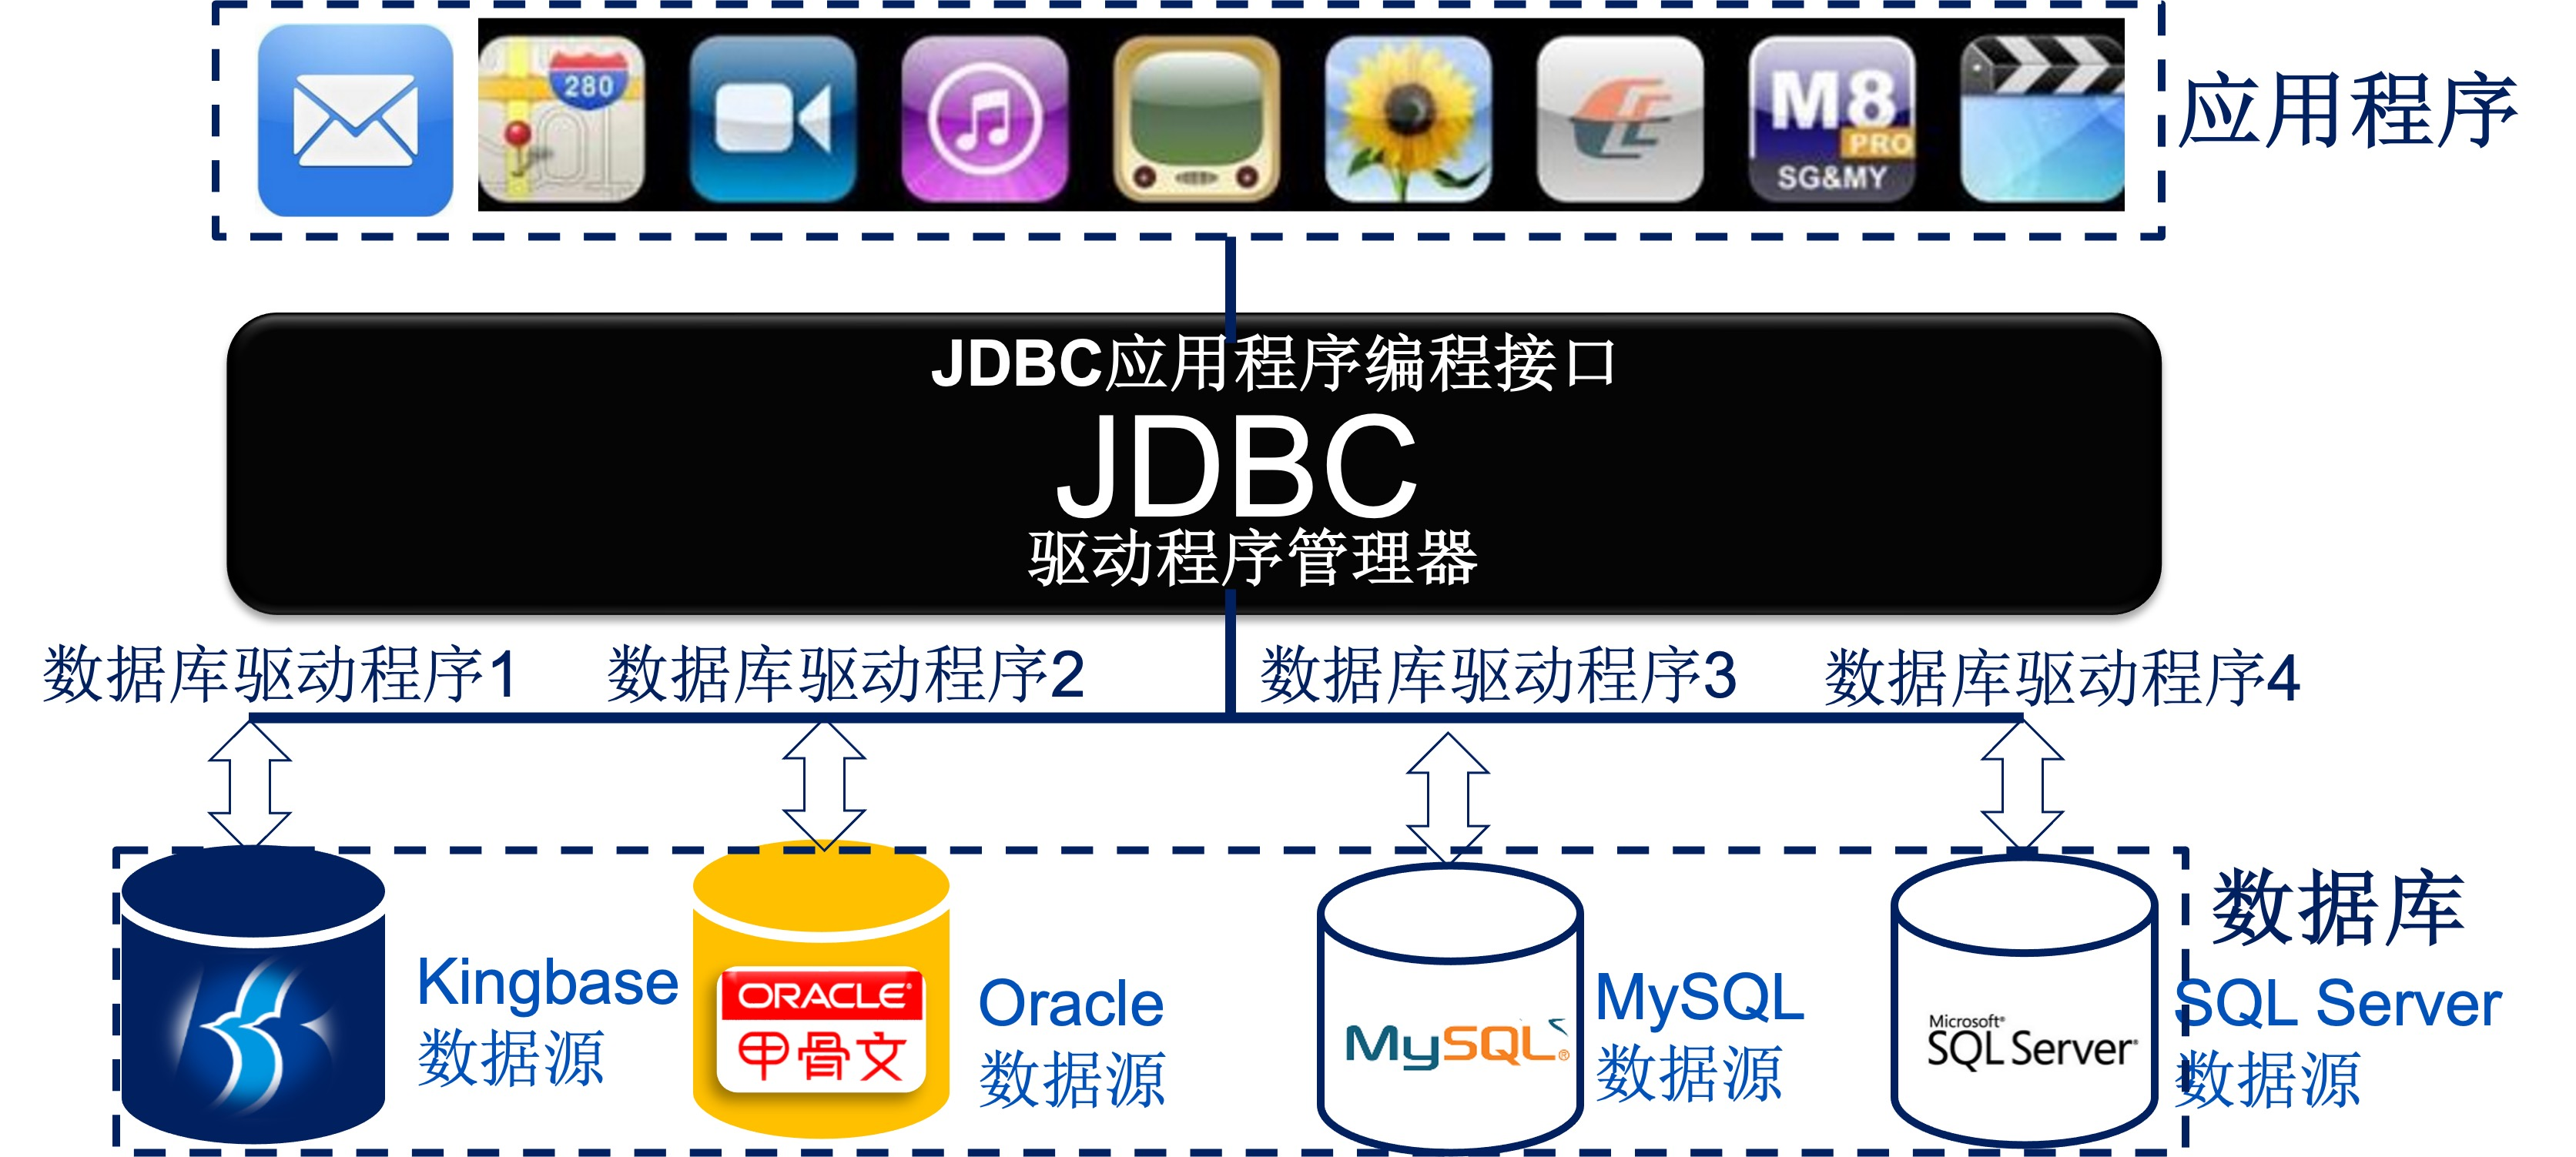
\includegraphics[width=0.9\textwidth]{figure/fig-10.jpg}
    \end{figure}
\end{itemize}
\end{frame}


\subsection{JDBC APIs基础}
\begin{frame}[allowframebreaks,fragile]{JDBC APIs基础}
\begin{itemize}
    \item JDBC中的常用类
    \begin{itemize}
        \item JDBC进行应用程序开发涉及到的所有类都包含在java.sql包中
        \item 不同的JDBC版本接口名和使用略有差异
    \end{itemize}
    \begin{figure}
        \centering
        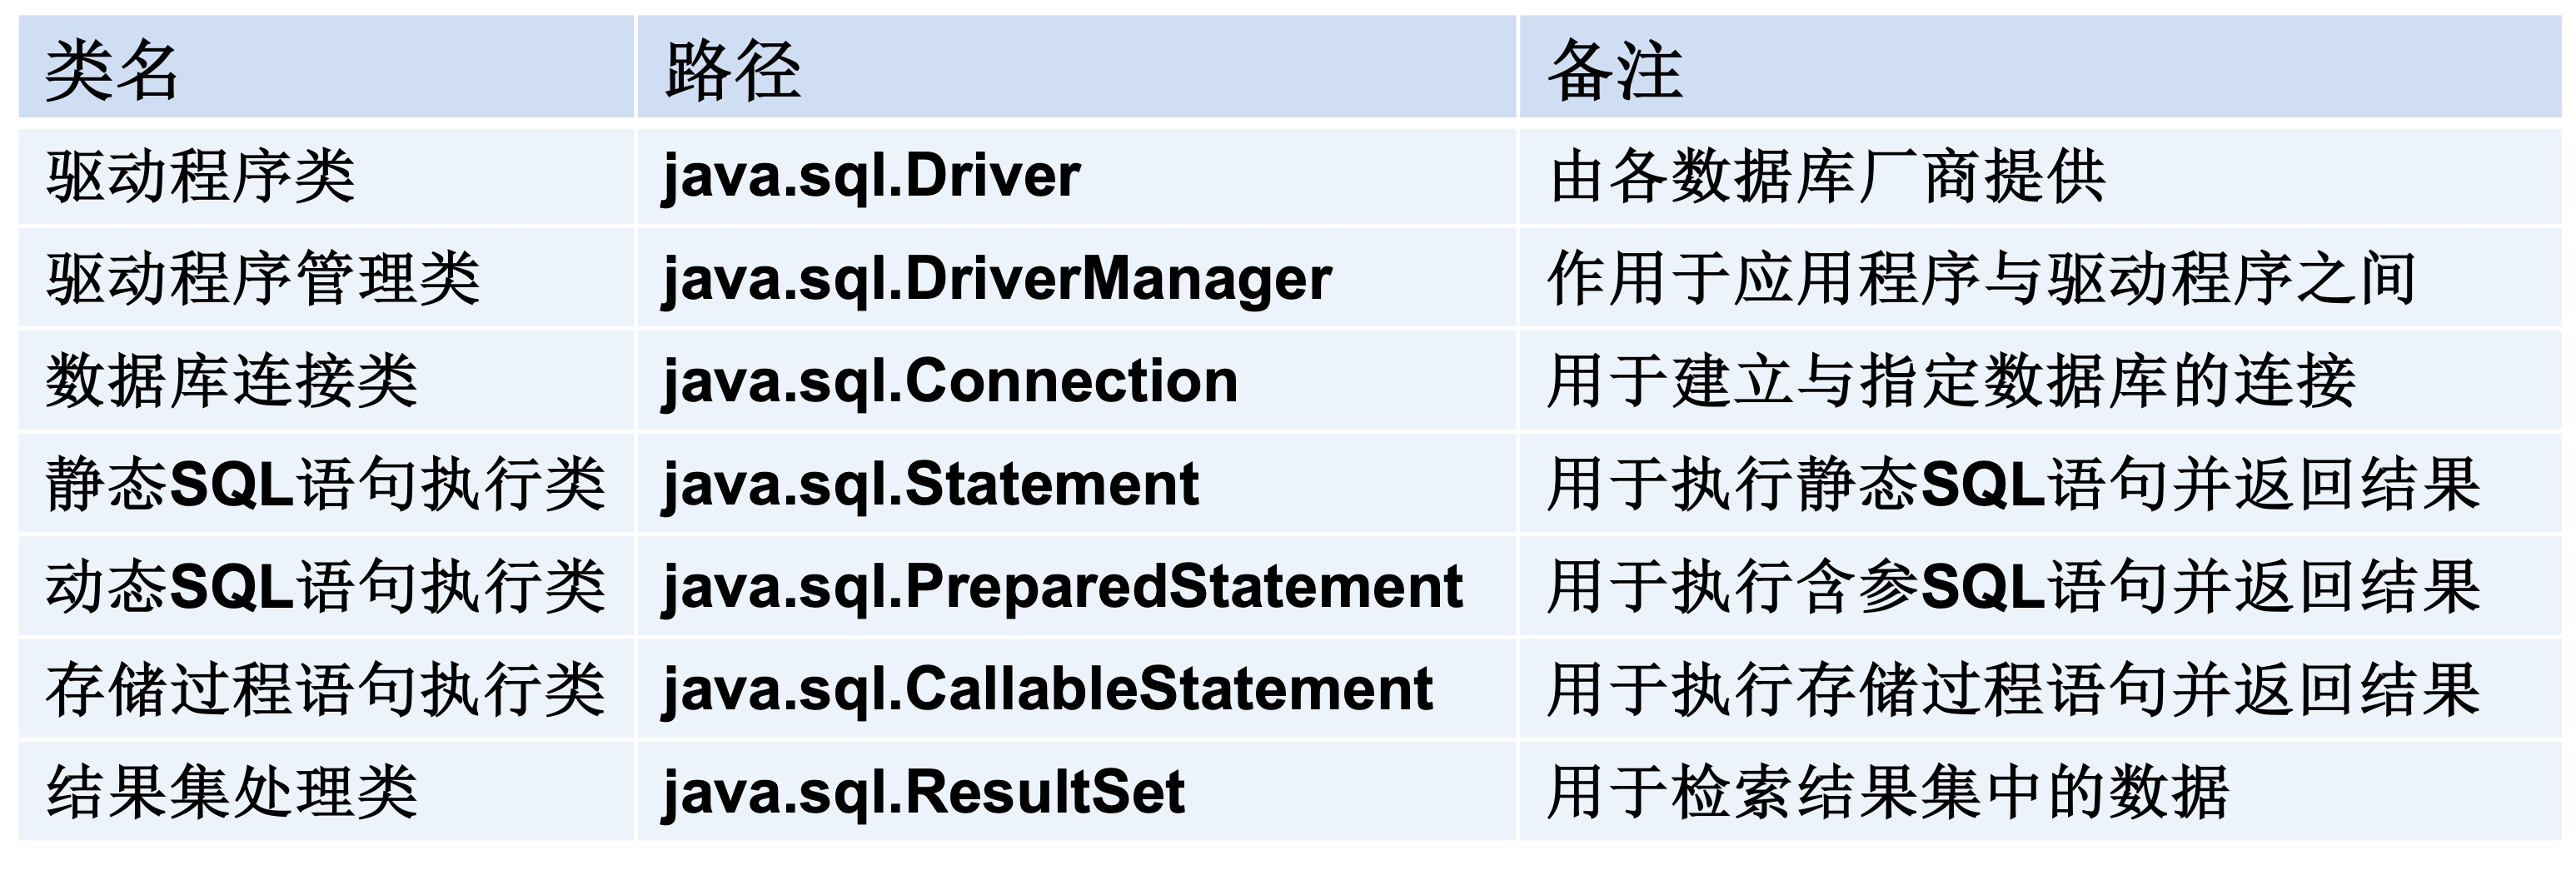
\includegraphics[width=0.9\textwidth]{figure/fig-11.jpg}
    \end{figure}
    \framebreak
    \item 数据类型
    \item 由数据库管理系统的驱动程序完成自身数据类型和JDBC标准数据类型的映射
    \begin{itemize}
        \item SQL数据类型:用于数据源
        \begin{itemize}
            \item VARCHAR、 CHAR 、 BIT 、NUMERIC、DATE等
        \end{itemize}
        \item Java数据类型:用于应用程序的Java代码
        \begin{itemize}
            \item String、boolean、BigDecimal、byte、short、int等
        \end{itemize}
    \end{itemize}
    
\end{itemize}
    \begin{table}[!htp]
        \centering
        \resizebox{0.7\textwidth}{!}{
        \begin{tabular}{c|c|c}
        \toprule
             & SQL数据类型 & Java数据类型 \\
        \midrule
             SQL数据类型 & 数据源之间转换 & 应用程序变量传递给语句 \\
            Java数据类型 & 从数据库中读取数据赋值给应用程序变量 & 应用程序变量之间转换\\
        \bottomrule
        \end{tabular}
        }
        \caption{SQL数据类型和java数据类型之间的转换规则}
        \label{tab:my_label}
    \end{table}
\end{frame}
\subsection{使用JDBC操纵数据库的工作流程}
\begin{frame}[allowframebreaks,fragile]{使用JDBC操纵数据库的工作流程}
\begin{enumerate}
    \item 步骤1:加载驱动程序
    \item 步骤2:建立与数据库的连接
    \begin{itemize}
        \item 定义连接的URL
        \item 利用生成的URL建立与数据库的连接
    \end{itemize}
    \item 步骤3:执行SQL语句
    \begin{itemize}
        \item 创建语句执行类对象
        \item 执行SQL语句,可以通过executeQuery、 executeUpdate、 execute三种方式执行
    \end{itemize}
    \item 步骤4:处理结果集
    \item 步骤5:释放资源
\end{enumerate}
\end{frame}


\begin{frame}[allowframebreaks,fragile]{使用JDBC操纵数据库的工作流程}
\begin{enumerate}
    \item 步骤1:加载驱动程序
    \begin{itemize}
        \item 驱动程序在JDBC API中实现定义数据交互的接口
        \item  【例8.7】对Kingbase、Oracle、SQL Server加载数据库驱动
\begin{block}{}
\begin{lstlisting}[language=Java, linewidth=\textwidth]
Class.forName("com.kingbase.Driver");       /* Kingbase */
Class.forName("oracle.jdbc.OracleDriver");  /* Oracle */
Class.forName(“com.microsoft.jdbc.sqlserver.SQLServerDriver”;   
/* SQL Server */
\end{lstlisting}
\end{block}
    \end{itemize}
\framebreak
    \item 步骤2:建立与数据库的连接
\begin{itemize}
    \item 加载驱动后,可以通过URL地址与数据库建立连接
    \item URL包含了连接数据库所需的协议、子协议和数据库名称,定义格式为:
    
    <协议名>:<子协议名>:<数据库名称>
    \item 【例8.8】定义与Kingbase、Oracle、SQL Server数据库连接的URL
\begin{block}{}
\begin{lstlisting}[language=Java, linewidth=\textwidth]
strURL = "jdbc:kingbase://" + 服务器名 +  ":" + 端口号 + "/" + 数据库名;
strURL = "jdbc:oracle:thin:@" + 服务器名 + ":" + 端口号 + ":" + 数据库名
strURL = "jdbc:microsoft:sqlserver://" + 服务器名 + ":" + 端口号 + ":" + 数据库名
// Kingbase、Oracle、SQL Server的默认端口号分别为54321、1521、1433
\end{lstlisting}
\end{block}
    \framebreak
    \item 【例8.9】建立与Kingbase数据库的连接,假定服务器地址为192.168.0.118,端口为54321,数据库名为DB-Student,用户名为Info001,密码为123456
    
\begin{block}{}
\begin{lstlisting}[language=Java, linewidth=\textwidth]
String strURL ="jdbc:kingbase:// 192.168.0.118:54321/DB-Student";
Connection conn= DriverManager.getConnection(strURL," Info001","123456");
\end{lstlisting}
\end{block}
\end{itemize}
    \framebreak
    \item 步骤3:执行SQL语句
    \begin{itemize}
        \item 静态语句执行类对象(Statement)
        \item 派生执行类对象:
            \begin{itemize}
                \item 动态语句执行类(PreparedStatement):执行动态的SQL语句
                \item 存储过程执行类(CallableStatement):执行数据库存储过程
            \end{itemize}
        \item 执行方法
            \begin{itemize}
                \item ResultSet executeQuery(): 执行数据库查询语句
                \item int executeUpdate(): 处理增、删、改以及定义语句
                \item boolean execute(): 处理存储过程或动态SQL语句
            \end{itemize}
        \item SQL注入防御
        \begin{itemize}
            \item 预编译
            \item 正则过滤,输入验证,框架......
        \end{itemize}
    \framebreak
        \item 【8.10】使用JDBC向课堂评价表中插入一条记录
\begin{block}{}
\begin{lstlisting}[language=Java, linewidth=\textwidth]
PreparedStatement stmt = conn.prepareStatement("INSERT INTO SC VALUES(?,?,?,?,?,?)");
/* 生成PreparedStatement类对象中的动态参数,注意第六个字段Feedback,未设置输入值 */
stmt.setString(1, " 20180001 ");    /*设置学生学号*/
stmt.setString(2, "19950018");  /*设置职工号*/
stmt.setString(3, "81001-01");  /*设置教学班号*/
stmt.setString(4, “老师讲得很出色");   /*设置学生评价意见*/
stmt.setBoolean(5,true);    /*设置学生评价意见类型*/
stmt.executeUpdate();
\end{lstlisting}
\end{block}    \end{itemize}


    \framebreak
    \item 步骤4:处理结果集
    \begin{itemize}
        \item ResultSet: 结果集合类对象
        \begin{itemize}
            \item .GetXXX(参数): 
        
            获取元组的属性值,XXX代表某种数据类型
            
            可以指定参数为列号(JDBC的列从1开始)或列名
            
            \item 游标(cursor):JDBC处理结果集的机制

            TYPE\_FORWARD\_ONLY:只能向下滚动(默认类型)
            
            TYPE\_SCROLL\_IN(SEN)SENSITIVE 双向滚动,区别为是否同步数据库更新操作
        \end{itemize}
    \framebreak
    \item 【8.12】遍历教师职工号为19950018,教学班号为81001-01的学生课程评价详情
\begin{block}{}
\begin{lstlisting}[language=Java, linewidth=\textwidth]
String SQL = "SELECT Sno, Assess, CAtype, Feedback FROM ClassAssess
  WHERE Tno='19950018' AND TCo = '81001-01'";
ResultSet rs = stmt.executeQuery(SQL);
while(rs.next()){
    String Sno = rs.getString("Sno");       /*等价于rs.getString(1)*/
    String strAssess = rs.getString("Assess");      /*等价于rs.getString(2) */
    Boolean bCAtype = rs.getBoolean ("CAtype");      /*等价rs.getBoolean (3) */
    String strFeedback = rs.getString("Feedback");  /*等价于rs.getString(4) */
    System.out.printf("[%s,%b,%s]%n", strAssess, bCAtype, strFeedback);
}
\end{lstlisting}
\end{block}


    \end{itemize}
  \framebreak
    \item 步骤5:释放资源
    \begin{itemize}
        \item 执行结束后,将与数据库进行交互的对象释放
        \item 释放资源有标准的顺序:
        \begin{itemize}
            \item 关闭结果集:ResultSet.close()
            \item 关闭语句执行类对象:Statement.close()
            \item 释放数据库连接对象:Connection.close()
        \end{itemize}
        \item 释放资源的Coding Tips
        \begin{itemize}
            \item Connection对象在应用程序中较为稀有,尽量做到晚创建,早释放
            \item 推荐在finally代码块中释放资源,以满足异常处理机制(finally语句在什么情况下都会执行,确保一定会释放资源)
        \end{itemize}
    \end{itemize}
\end{enumerate}
\end{frame}

\begin{frame}[allowframebreaks,fragile]{【例8.13】基于JDBC实现【任务4】}
\begin{columns}
\begin{column}{0.6\textwidth}
\vspace{-2ex}
\begin{itemize}
    \item 选课关系模式:
    \begin{itemize}
        \item SC(Sno,TCno, Grade)
    \end{itemize}
    \vspace{-1ex}
    \item 教师关系模式:
    \begin{itemize}
        \item Teacher(Tno, Tname, Ttitle, Tbirthdate, Dno)
    \end{itemize} 
    \vspace{-1ex}
    \item 教学班关系模式: 
    \begin{itemize}
        \item TeachingClass(TCno, Capacity, Semester, Cno)
    \end{itemize}
    \vspace{-1ex}
    \item 讲授关系模式:
    \begin{itemize}
        \item Teaching(TCno, Tno, isLeading) 
    \end{itemize}
    \vspace{-1ex}
    \item 课堂评价关系模式: 
    \begin{itemize}
        \item ClassAssess(Sno, Tno, TCno, Assess, CAtype, CRfeedback)
    \end{itemize}
\end{itemize}
\end{column}

\begin{column}{0.4\textwidth}
\begin{figure}
    \centering
    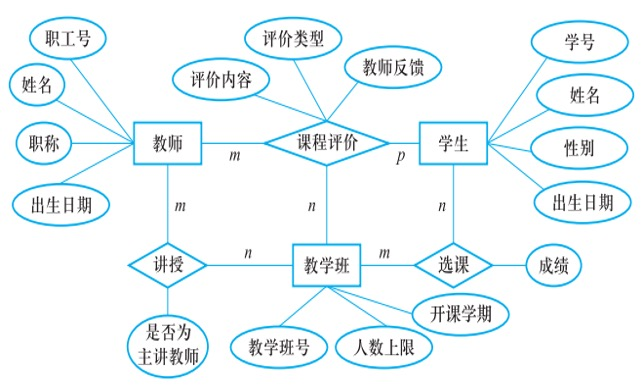
\includegraphics[width=\textwidth]{figure/fig-14.jpg}
\end{figure}
\end{column}

\end{columns}
\end{frame}


\begin{frame}[allowframebreaks,fragile]{【例8.13】基于JDBC实现【任务4】}
\begin{columns}
\begin{column}{0.4\textwidth}
\vspace{-2ex}
\begin{itemize}
    \item 数据库连接的管理
    \begin{itemize}
        \item 设置连接数据库的URL
        \item 创建连接数据库的静态函数
        \item 创建释放数据库连接对象的静态函数
    \end{itemize}
    \item 封装(步骤1-步骤2-步骤6)到数据库连接管理类中
\end{itemize}
\end{column}

\begin{column}{0.6\textwidth}
\vspace{-4ex}
\begin{block}{}
\begin{lstlisting}[language=Java, linewidth=\textwidth, basicstyle=\ttfamily\tiny]
public class ConnectionManager{
    static final String jdbcUrl="jdbc:kingdb://192.168.0.118:54321/DB-Student";
    static final String jdbcUsername = "Info001";
    static final String jdbcPassword = " 123456";
    private static Connection connection = null;
    /* 静态代码段, 加载Kingbase数据库驱动程序 */
    static {
        Class.forName("com.kingbase.Driver");
    }
    public static Connnection createConnection(){
        connection = DriverManager.getConnection(jdbcUrl, jdbcUsername, jdbcPassword);
        System.out.println("数据库连接成功");
        return connection;
    }
    /* 释放资源 */
    public static void release(){
        if (connection != null) connection.close();
        System.out.println("释放资源成功");
    }

}
\end{lstlisting}
\end{block}
\end{column}

\end{columns}
\end{frame}


\begin{frame}[allowframebreaks,fragile]{【例8.13】基于JDBC实现【任务4】}
\begin{columns}
\begin{column}{0.4\textwidth}
\vspace{-2ex}
\begin{itemize}
    \item 学生浏览指定的教学班和授课教师,并输入课程评价
    \item 完成步骤3-4
    \item 步骤3:创建语句对象
    \item 步骤4:执行语句对象
\end{itemize}
\end{column}

\begin{column}{0.6\textwidth}
\vspace{-4ex}
\begin{block}{}
\begin{lstlisting}[language=Java, linewidth=\textwidth, basicstyle=\ttfamily\tiny]
Connection conn = ConnectionManager.createConnection();
Statement stmnt = conn.createStatement();
/* 设置如下任务的SQL语句;获取学生所选的教学班及授课老师 */
/* 假设strSno为学生学号 */
String SQL4ClassAssess = "SELECT TCno, Tno FROM Student, Teacher, Teaching, SC WHERE Teacher.Tno=Teaching.Tno AND Teaching.TCno=SC.TCno AND SC.sno="+strSno;                          
\end{lstlisting}
\end{block}
\end{column}

\end{columns}
\end{frame}


\begin{frame}[allowframebreaks,fragile]{【例8.13】基于JDBC实现【任务4】}
\begin{columns}
\begin{column}{0.4\textwidth}
\vspace{-2ex}
\begin{itemize}
    \item 执行步骤5
    \begin{itemize}
        \item 根据结果集,执行用户的逻辑
        \item 构建学生课程评价的动态SQL语句
        \item 遍历学生选课的每一条记录,在动态SQL语句中设置学生对该门课程的评价,并更新该条记录
    \end{itemize}
    \item 执行步骤6
    \begin{itemize}
        \item 释放结果集、语句、连接对象
    \end{itemize}
\end{itemize}
\end{column}

\begin{column}{0.6\textwidth}
\vspace{-4ex}
\begin{block}{}
\begin{lstlisting}[language=Java, linewidth=\textwidth, basicstyle=\ttfamily\tiny]
ResultSet rs=stmnt.executeQuery(SQL4ClassAssess);
/* 设置插入学生课程评价的动态SQL语句 */
String insertSQL = "INSERT INTO ClassAssess(Sno, Tno, TCno, Assess, CAtype) VALUES(?,?,?,?,?)";
PreparedStatement ps = conn.prepareStatement(insertSQL);
while(rs.next){
    /* 阅读该学生所选的教学班及授课老师 */
    String strTno = rs.getString("Tno");
    String strTCno = rs.getString("TeachingClassNo");
    /* 对该授课教师讲授的教学班进行评价 */
    ps.setString(1, strSno);
    ps.setString(2, strTno);
    ps.setString(3, strTeachingClassNo);
    ps.setString(4, "老师讲得很好");
    /* 课程评价根据用户输入 */
    ps.setBoolean(5, true);
    ps.executeUpdate();
}
rs.close();
ps.close();
stmnt.close();
ConnectionManager.release();
\end{lstlisting}
\end{block}
\end{column}

\end{columns}
\end{frame}


\section{基于MVC框架的数据库应用开发}
\subsection{基于MVC框架的数据库应用开发}

\begin{frame}[allowframebreaks,fragile]{什么是MVC}
\begin{columns}
\begin{column}{0.4\textwidth}
\begin{itemize}
    \item MVC框架包含三个部分每个部分各自处理自己的工作,互不干扰
    \begin{itemize}
        \item 业务模型控制器 (Controller)
        \item 业务模型 (Model)
        \item 用户结果呈现 (View)
    \end{itemize}
\end{itemize}
\end{column}

\begin{column}{0.6\textwidth}
\begin{figure}
    \centering
    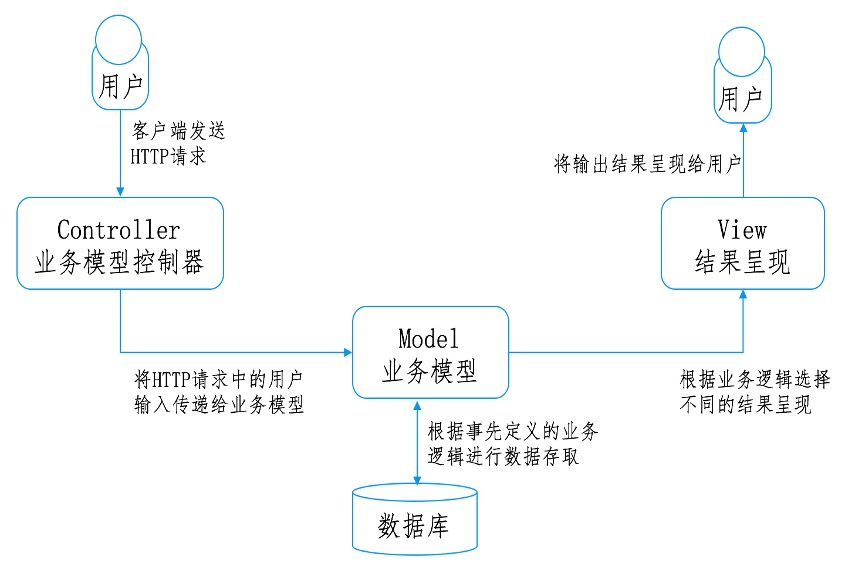
\includegraphics[width=\textwidth]{figure/fig-15.jpg}
\end{figure}
\end{column}

\end{columns}
\end{frame}


\begin{frame}[allowframebreaks,fragile]{什么是MVC}
\begin{columns}
\begin{column}{0.4\textwidth}
\begin{itemize}
    \item \textcolor{red}{业务模型控制器}:接收用户通过浏览器发送的HTTP服务请求
    \begin{itemize}
        \item 包括用户需要选择的业务模型,以及其它可选的输入参数
        \item 可以是用户在文本框中输入的文本、下拉列表框中的数据项等
        \item 也可以是用户的操作类型
    \end{itemize}
\end{itemize}
\end{column}

\begin{column}{0.6\textwidth}
\begin{figure}
    \centering
    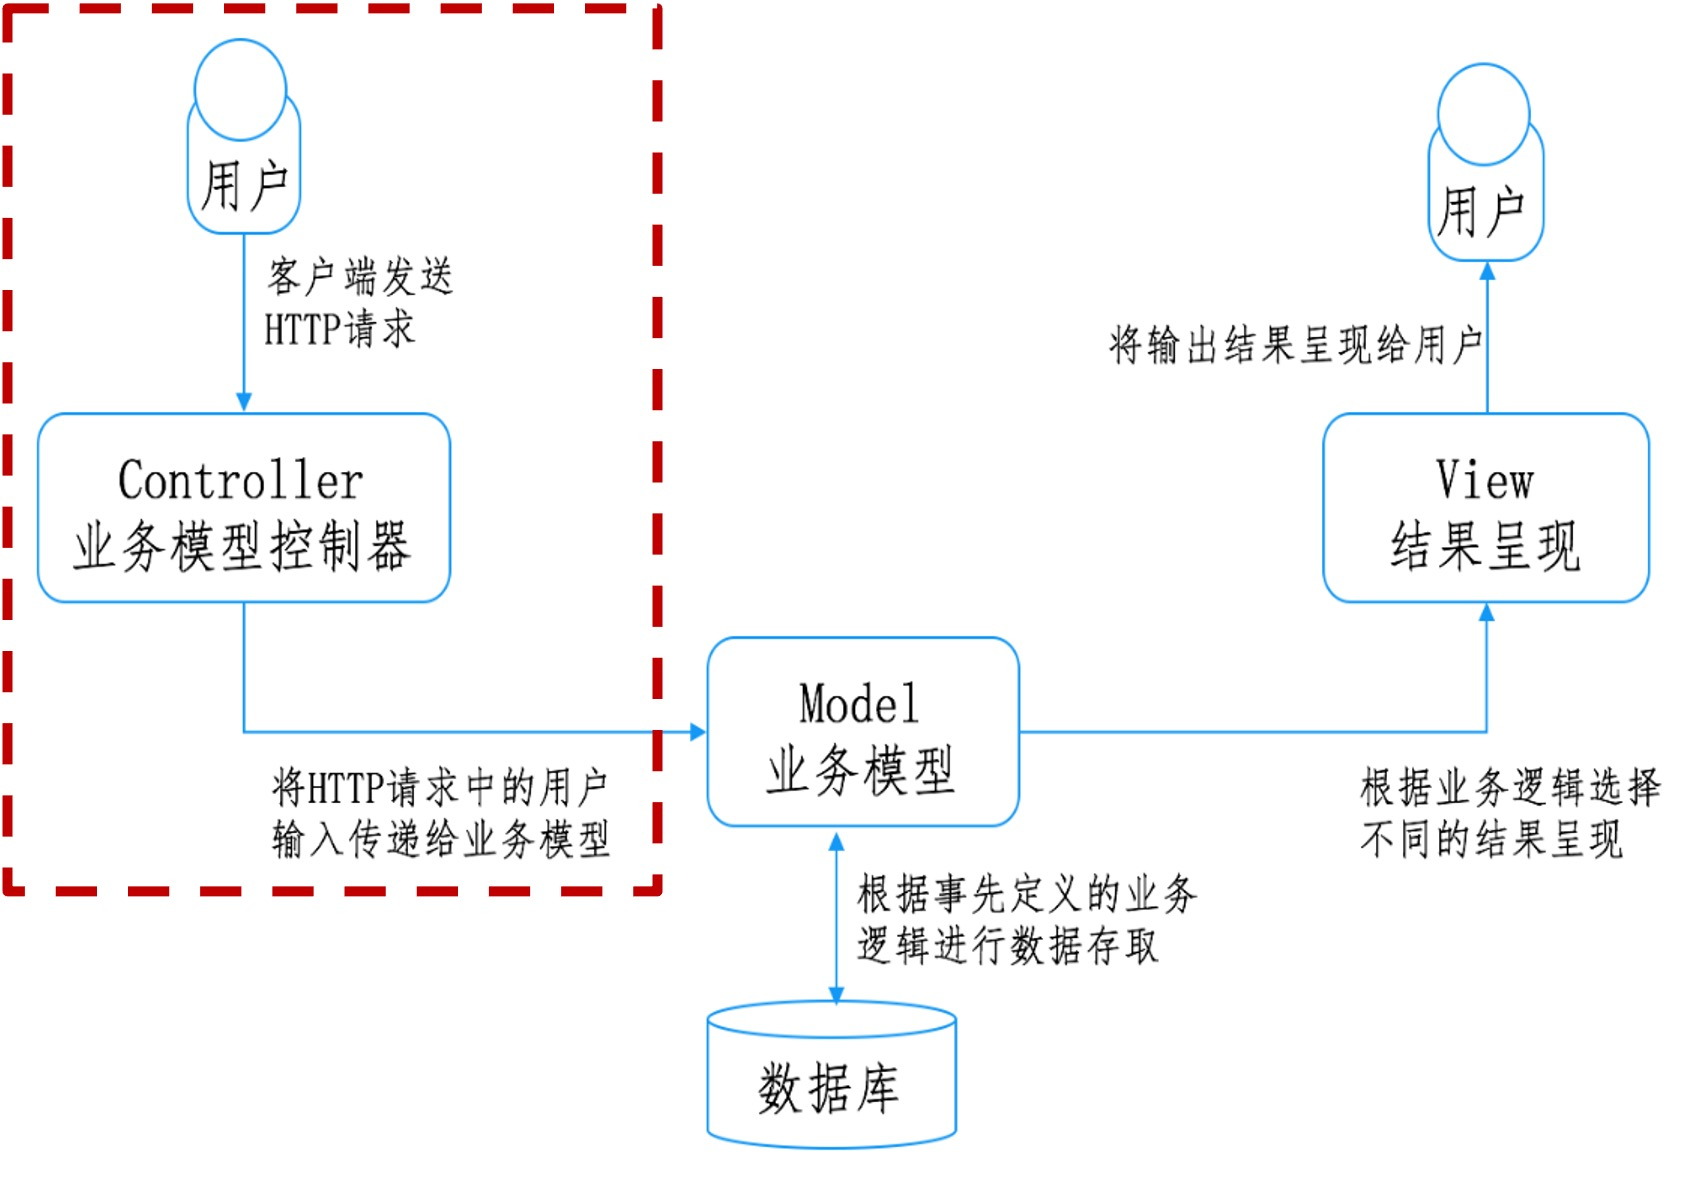
\includegraphics[width=\textwidth]{figure/fig-16.jpg}
\end{figure}
\end{column}

\end{columns}
\end{frame}


\begin{frame}[allowframebreaks,fragile]{什么是MVC}
\begin{columns}
\begin{column}{0.4\textwidth}
\begin{itemize}
    \item \textcolor{red}{业务模型}:建立用户的业务逻辑
    \begin{itemize}
        \item 解析出来的用户数据,执行事先定义的业务逻辑,并操纵数据库存取数据
        \item 输出独立于具体的数据格式,可为多个用户结果呈现提供展示所需要的数据,减少了代码的重复性
    \end{itemize}
\end{itemize}
\end{column}

\begin{column}{0.6\textwidth}
\begin{figure}
    \centering
    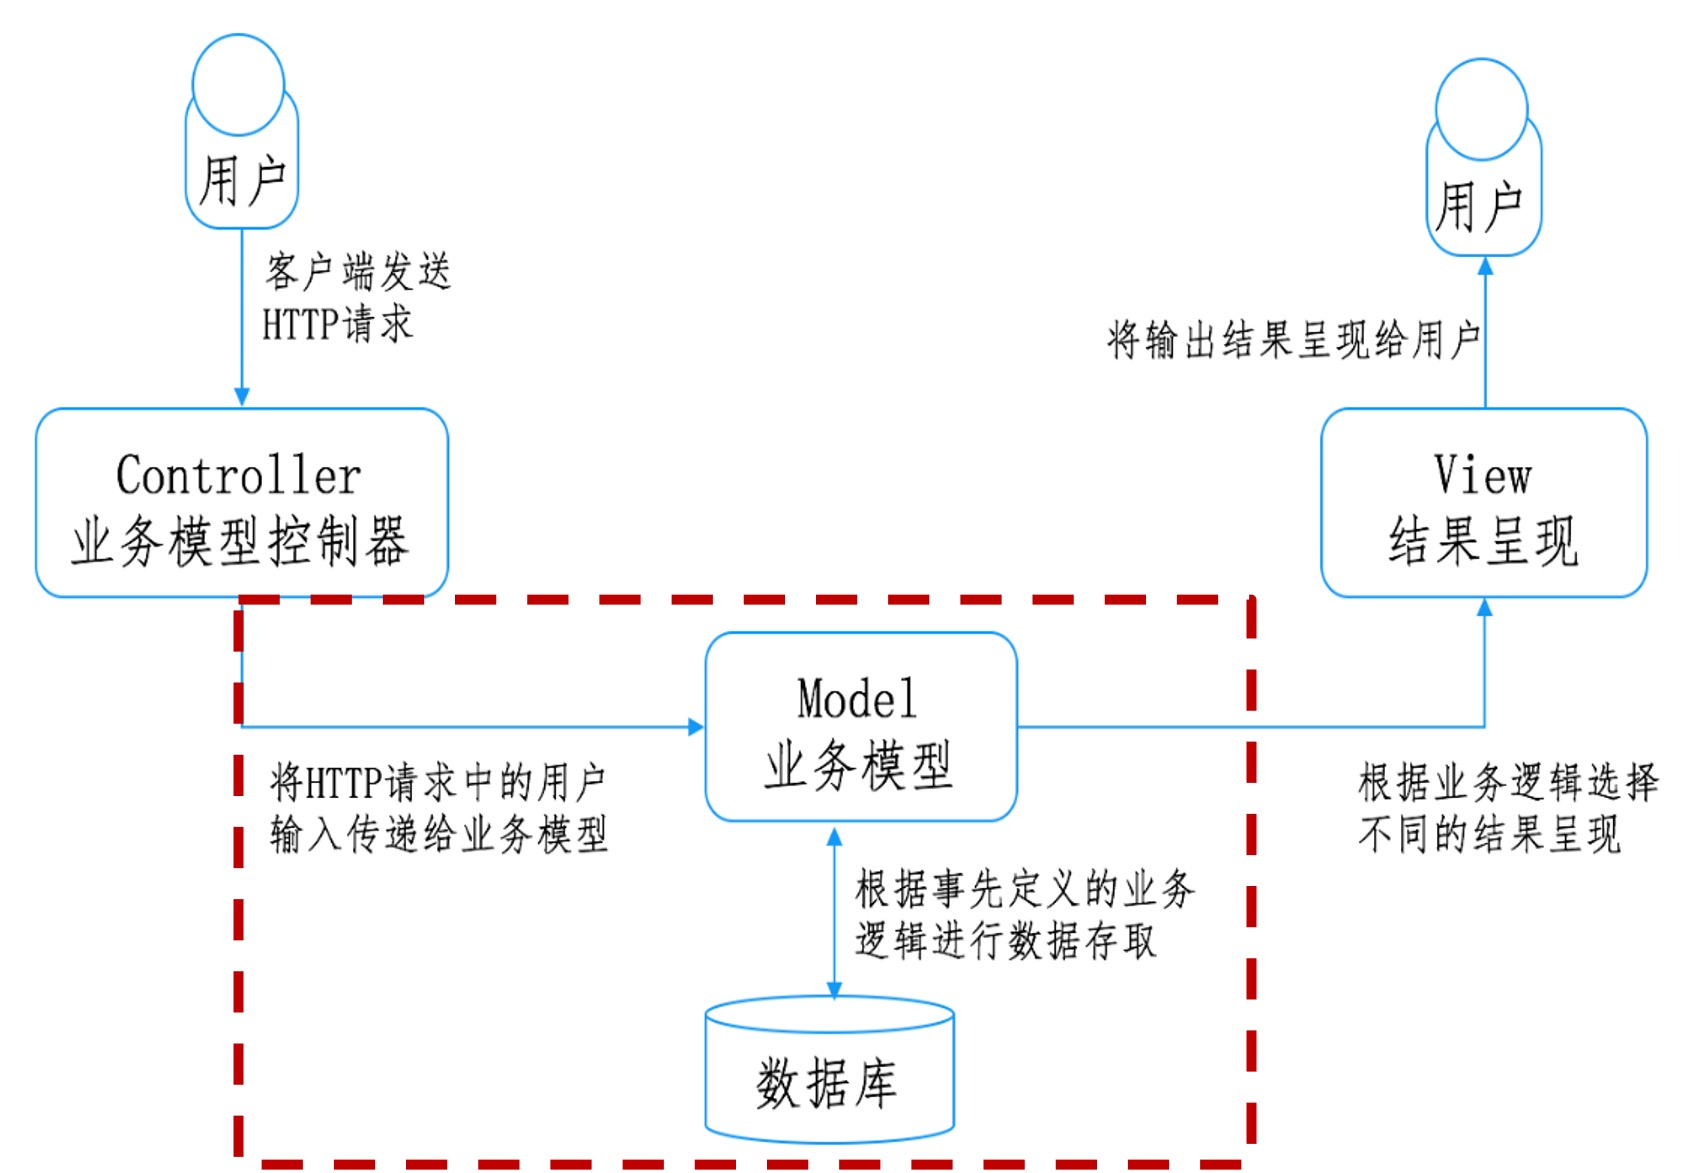
\includegraphics[width=\textwidth]{figure/fig-17.jpg}
\end{figure}
\end{column}

\end{columns}
\end{frame}


\begin{frame}[allowframebreaks,fragile]{什么是MVC}
\begin{columns}
\begin{column}{0.4\textwidth}
\begin{itemize}
    \item \textcolor{red}{用户结果呈现}:用户看到并与之交互获得结果展示的界面
    \begin{itemize}
        \item 根据业务模型输出的结果反馈给客户端进行呈现
    \end{itemize}
\end{itemize}
\end{column}

\begin{column}{0.6\textwidth}
\begin{figure}
    \centering
    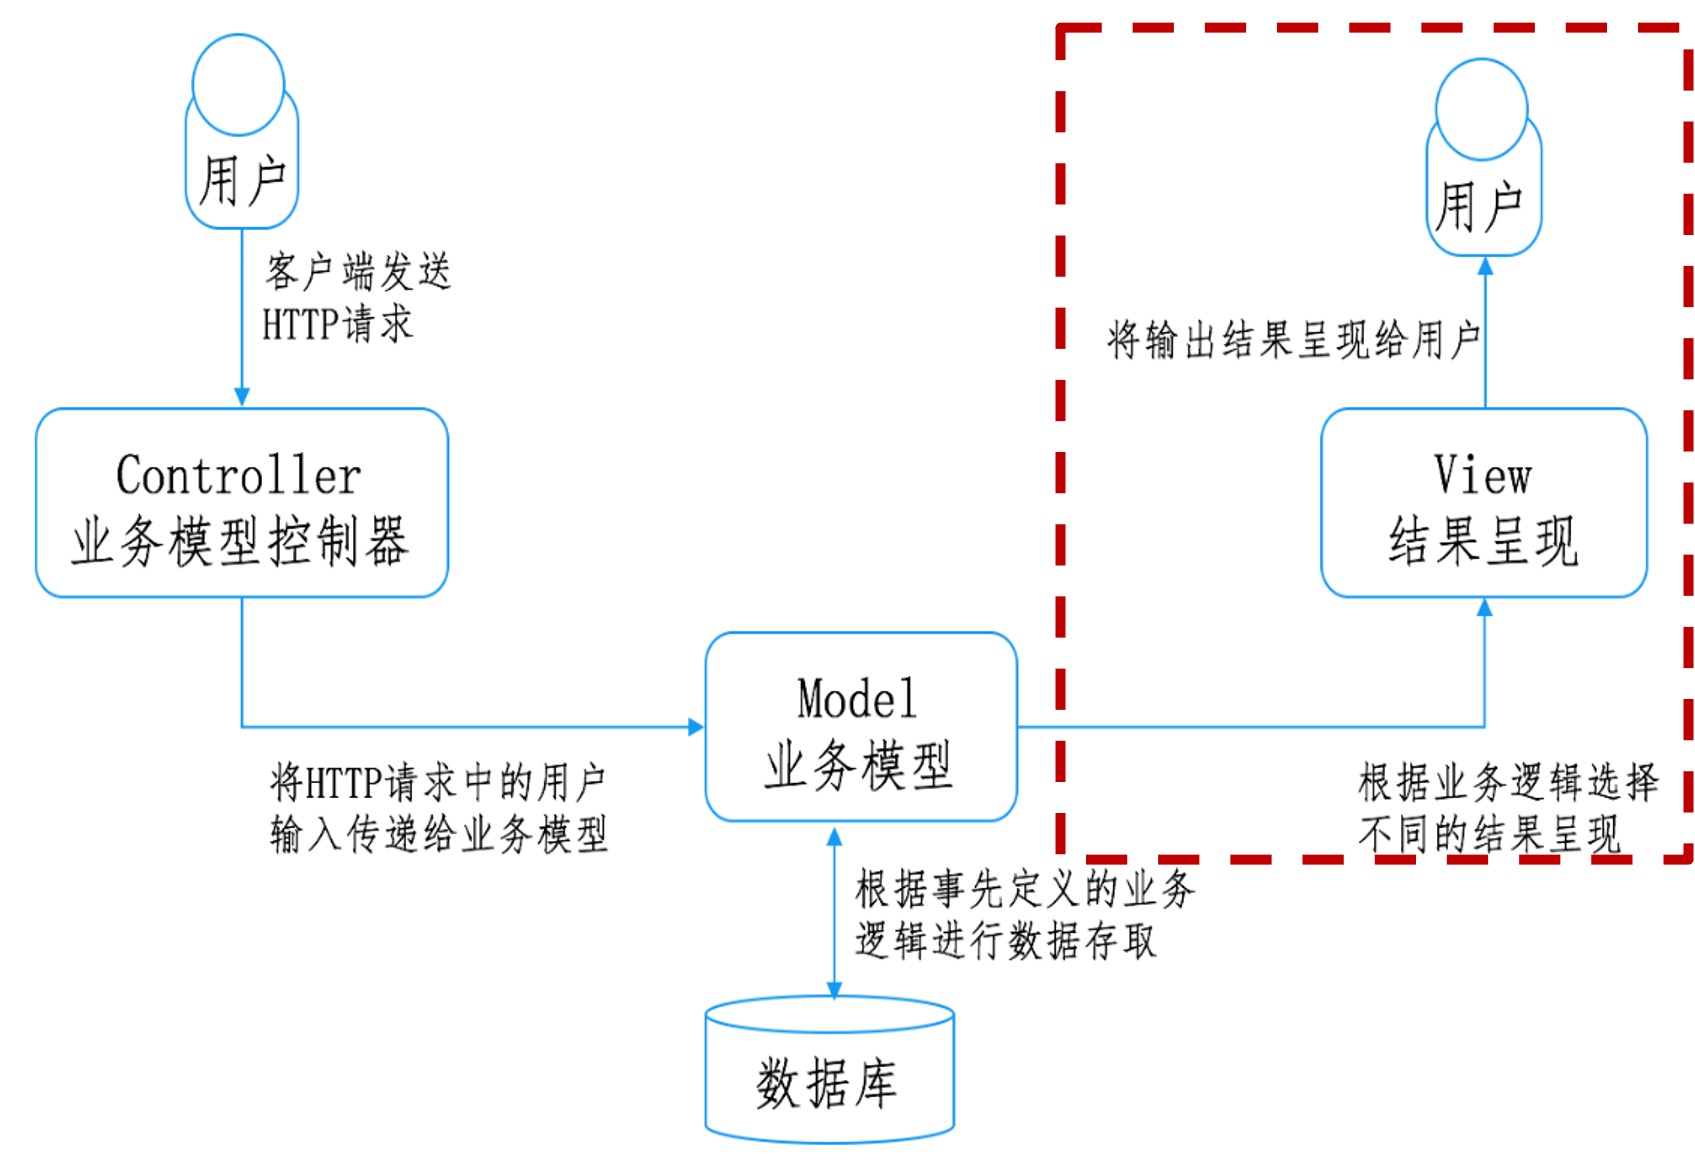
\includegraphics[width=\textwidth]{figure/fig-18.jpg}
\end{figure}
\end{column}

\end{columns}
\end{frame}



\begin{frame}[allowframebreaks,fragile]{使用MVC框架实现任务4的系统流程图}
\begin{figure}
    \centering
    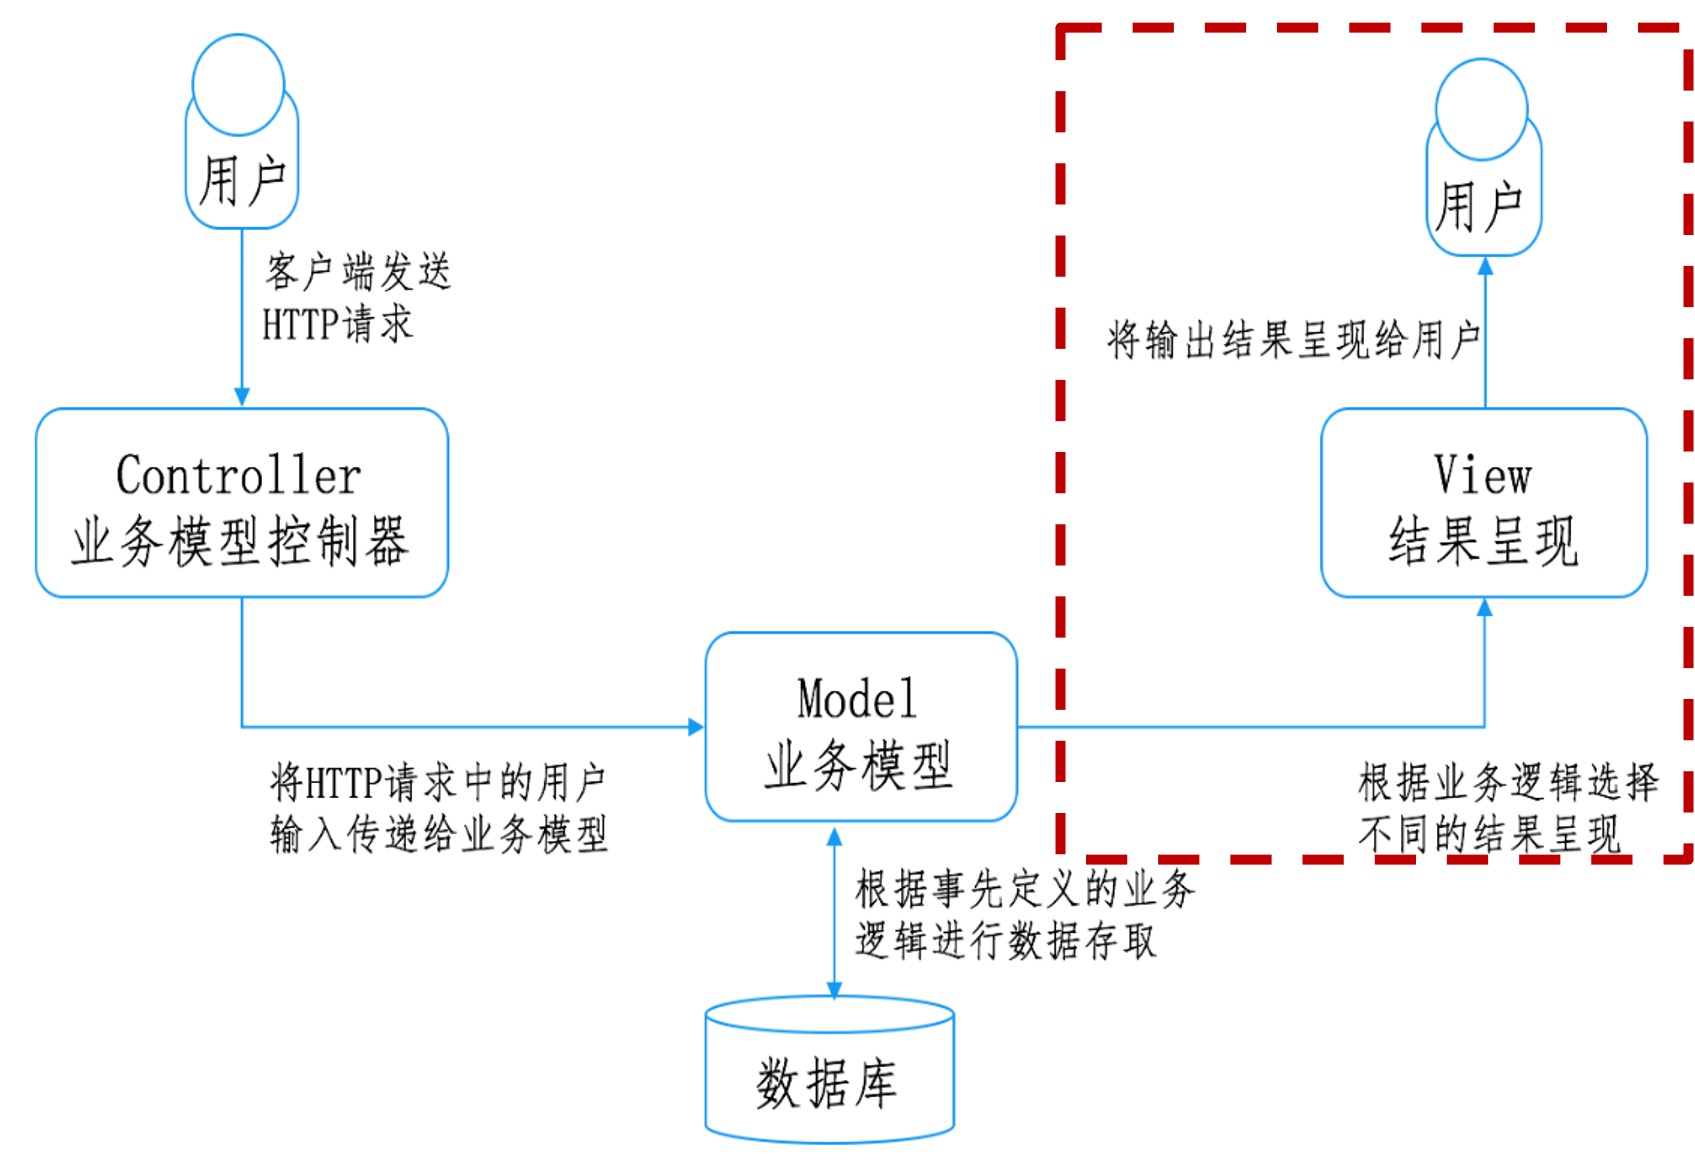
\includegraphics[width=\textwidth]{figure/fig-18.jpg}
\end{figure}

\end{frame}


\section{本章小结}
\begin{frame}{本章小结}
\begin{itemize}
    \item 扩展SQL语言的功能
    \begin{itemize}
        \item 引入新的SQL子句、引入新的内置函数、引入PL/SQL以及存储过程和存储函数等技术
        \item SQL与高级语言具有不同的数据处理方式。SQL是面向集合的,而高级语言是面向记录的。游标就是用来协调这两种不同的处理方式的机制
    \end{itemize}


    \item 通过高级语言实现复杂应用
    \begin{itemize}
        \item JDBC的工作原理和工作流程
        \item 基于MVC框架的开发方式
    \end{itemize}


\end{itemize}
    
\end{frame}

\backmatter

\begin{frame}[t]
\frametitle{Reference}
\framesubtitle{参考资料}
\nocite{*}
\bibliographystyle{abbrvnat} % We choose the "plain" reference style
\bibliography{refs}
\end{frame}

\end{document}
